\documentclass{report}
\usepackage{filecontents}

\usepackage[utf8]{inputenc}
\usepackage[T1]{fontenc}
\usepackage[francais]{babel}
\usepackage{listings}
\usepackage[a4paper]{geometry}
\usepackage{graphicx}
\usepackage[export]{adjustbox}
\usepackage{titlesec}
\usepackage{color}
\usepackage[toc, page]{appendix}
\usepackage{url}

\definecolor{xcodekw}{rgb}{0.75, 0.22, 0.60}
\definecolor{xcodestr}{rgb}{0.89, 0.27, 0.30}
\definecolor{xcodecmt}{rgb}{0.31, 0.73, 0.35}

\titleformat{\chapter}[display]
  {\centering\normalfont\huge\bfseries}
  {\chaptertitlename\ \thechapter}
  {20pt}
  {\Huge}

\geometry{hscale=0.75,vscale=0.85,centering}

\renewcommand{\thesection}{\arabic{section}}
\renewcommand\appendixtocname{Annexes}
\renewcommand\appendixname{Annexes}
\renewcommand\appendixpagename{Annexes}

\title{Sécurité des Réseaux Informatiques\\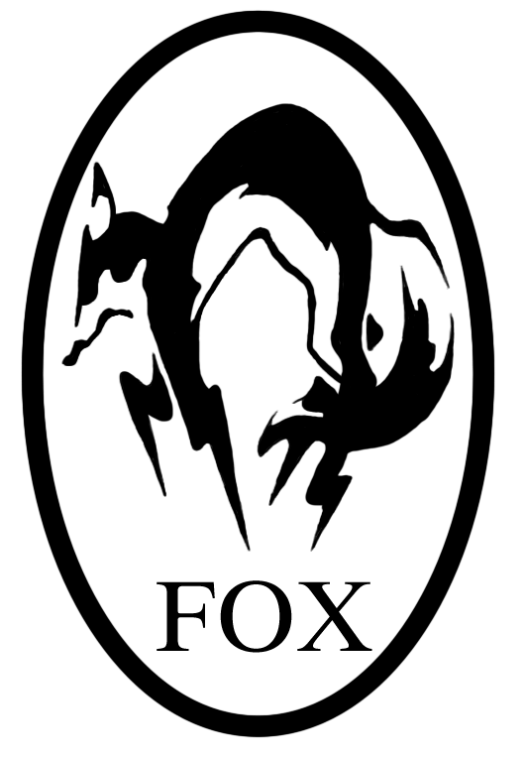
\includegraphics[scale=0.3]{foxhound.png}}
\author{Micouille "The Boss" \bsc{Riffon} \& Samuel "Big Boss" \bsc{Monroe}}

\date{30 Mai 2015}

\begin{document}

\maketitle

\newpage
\thispagestyle{empty}
\mbox{}

\tableofcontents

%% \textbf{}

\chapter{Avant-propos}

	\section{The Boss}

		Si toi aussi ça te casse bien les couilles d'étudier dans des slides où les informations importantes concernant un sujet sont répartis sur 10-15 slides différents, voici le document qu'il te faut.\\

		Sois redevable aux membres de F0XHOUND, toi qui galère à travailler sur une autre matière que TDS car on a presque quedalle à étudier cette année.\\

		Ce document reprendra donc la matière non reprise dans le syllabus \textbf{mais} présente dans les slides (les 10-11-12). Et je précise que ce document reprend exactement la matière des slides avec parfois des précisions en plus dans la mesure du possible.


	\section{Big Boss}

		Ceci ne consitue pas une synthèse, mais plutôt une oeuvre composée de mes notes prises en cours, et de la réunion du syllabus de V.Van den Schrieck ainsi que du livre Computer Security de Stallings.\\

		Le but est d'obtenir une compréhension totale du cours à la première lecture et d'offrir aux membres de Fox Hound les compétences qui sont attendues d'eux, afin de pouvoir pérenniser ce groupe et ses objectifs.\\

\chapter{Généralités}

	Identification des différents concepts et principes de la sécurité informatique.\\

	\section{Concepts de sécurité informatique}

		\textbf{Sécurité Informatique} : Protection fournie à un SI automatisé pour atteindre les objectifs de préservation \textbf{CIA} des ressources (matériel, logiciels, données, etc..) du SI.\\

		\textbf{CIA} est un concept clé dans la sécurité : \\

		\begin{itemize}
			\item \textbf{Confidentiality} : Préserve les autorisations et restrictions sur l'accès à l'information ainsi que sur la vie privée.\\
			\item \textbf{Integrity} : Protection contre la modification ou suppression impropre de données, incluant l'assertion de l'authenticité des données.\\
			\item \textbf{Availability} : Assure la disponibilité et accessibilité sûre aux données et services.\\
		\end{itemize}

		Ces trois concepts forment la triade \textbf{CIA}, aussi représentée en triangle, et indique les trois objectifs de préservation des assets (\textbf{data} \& \textbf{services}).\\
		Cette triade peut être additionnée de deux autres concepts : \\

		\begin{itemize}
			\item \textbf{Authenticity} : Propriété d'être authentique, et capable d'être vérifié et digne de confiance.\\
			\item \textbf{Accountability} : Besoin de pouvoir tracer les actions à des fins d'identification.\\
		\end{itemize}

	\section{Terminologie}

		Voyons ici quelques termes reliés à la sécurité qu'il est nécéssaire de maîtriser : \\

		\subsection{Asset}

			Les assets, ressources, sont des éléments que les utilisateurs ou propriétaires souhaitent protéger.\\

			Les assets peuvent être \textbf{hardware}, \textbf{software}, \textbf{données} et \textbf{réseux et moyens de communications}. Des ressources non physiques telles que la \textbf{réputation} doivent également être prises en compte.\\

		\subsection{Security Policy}

			Une \textbf{politique de sécurité} est un ensemble de règles ou pratiques qui spécifient ou régulent la manière dont un système ou organisation fournit des services de sécurité pour protéger les \textbf{assets}.\\

			Composée de \textbf{contre-mesures}, ensemble de \textbf{règles} et de \textbf{procédures}.\\

		\subsection{Vulnerability}

			Faille ou faiblesse dans la conception, implémentation, opération ou gestion d'un système, qui peut être \textbf{exploitée} pour violer la \textbf{security policy}.\\

			Ces vulnérabilités peuvent être la \textbf{corruption système} (I) , des \textbf{fuites} (C) ou des \textbf{indisponibilités} (A).\\

		\subsection{Threats and Attacks}

			Une \textbf{menace} est un danger potentiel de sécurité pour une ressource.\\

			L'\textbf{attaque} est la réalisation de ce danger potentiel.\\
			Elles peuvent êtres \textbf{actives} ou \textbf{passives} selon qu'elles altèrent le système ou non, et \textbf{internes} ou \textbf{externes} selon la position de l'attaquant par rapport à l'entreprise.\\

		\subsection{Countermeasures}

			La \textbf{contremesure} est une action visant à réduire une menace, vulnérability ou attaque via prévention, élimination.\\

		\subsection{Risk}

			Le \textbf{risque} est la prévision d'une perte exprimée par la probabilité qu'une menace particulière exploire une vulnérabilité particulière avec un résultat négatif particulier.\\

			Un risque est \textbf{évalué} par la \textbf{probabilité que l'incident} survienne multiplié par \textbf{l'impact} que cet incident causerait.\\

	\section{Menaces, attaques et actifs}

		\subsection{Divulgation non autorisée - Unauthorised Disclosure}

			Menace sur \textbf{Confidentiality}, attaques liées : \\

			\begin{itemize}
				\item \textbf{Exposition} : Exposition d'informations sensibles
				\item \textbf{Interception} : Interception d'informations dans une communication
				\item \textbf{Inférence} : Accession à des infos sensibles de manière indirecte
				\item \textbf{Intrusion}\\
			\end{itemize}

		\subsection{Tromperie - Deception}

			Transmission de fausses infos à une entité en faisant croire que les infos sont conformes. \\

			\begin{itemize}
				\item \textbf{Masquerade} : Accès au système et agissement malicieux sous couvert d'une entité autorisée
				\item \textbf{Falsification} : Alteration de données valides
				\item \textbf{Répudiation}\\
			\end{itemize}

		\subsection{Perturbations - Disruptions}

			Menaces sur \textbf{Availability} et \textbf{Integrity}.\\

			\begin{itemize}
				\item \textbf{Neutralisation} : Destruction physiques ou endommagement du matériel
				\item \textbf{Corruption}
				\item \textbf{Obstruction} : Interruption d'un service, DoS\\
			\end{itemize}

		\subsection{Usurpation}

			Prise de contrôle d'un service ou système par une entité non autorisée.\\

			\begin{itemize}
				\item \textbf{Détournement} : Entité contrôle les ressoruces d'un système
				\item \textbf{Mauvais usage} : Composant système effectue une opération au détriment de la sécurité.\\
			\end{itemize}

	\section{Principes de conception de systèmes sécurisés}

		Pas de techniques pour empêcher totalement des \textbf{failles}, mais des principes existent pour tendre vers un \textbf{système sécurisé} : \\

		\begin{itemize}
		 	\item \textbf{Economy of Mechanisms} : Solutions les moins complexes possibles pour éviter les failles (\textbf{KISS}).\\
		 	\item \textbf{Fail-Safe Default} : Comportement d'exclusion par défault
		 	\item \textbf{Complete Mediation} : Chaque accès système doit être validé, pas de caches
		 	\item \textbf{Open Design} : Elements de conception publiques
		 	\item \textbf{Separation of Privilege}
		 	\item \textbf{Least Privilege} : Droits minimum suffisant pour la tâche
		 	\item \textbf{Least Common Mechanisms} : Il faut minimiser les éléments partagés par les différents programmes ou utilisateurs.
		 	\item \textbf{Psychological Acceptability} : Les mécanismes de sécurité ne doivent pas interférer sans raison avec les tâches des users, qui pourraient les désactiver.
		 	\item \textbf{Isolation} : Systèmes publiques isolés des critques, processus et fichiers utilisateurs isolés de ceux des autres, accès aux mécanismes isolés
		 	\item \textbf{Encapsulation} : Isolation appliquée à l'orienté-objet
		 	\item \textbf{Modularity} : Partage des fonctions et services de sécurité pour une seule implémentation d'un prtocole de sécurité.
		 	\item \textbf{Layering} : Plusieurs couches de protection
		 	\item \textbf{Least Astonishment} : Une GUI doit se comporter comme l'attendrait un utilisateur\\
		 \end{itemize} 

	\section{Stratégies de sécurité informatique}

		Trois étapes pour mettre au point une stratégie : \\

		\begin{enumerate}
			\item \textbf{Définir} la politique de sécurité
			\item \textbf{Implémenter} la politique
			\item \textbf{Valider} la politique\\
		\end{enumerate}

		\subsection{Politiques de sécurité}

			Il faut dans un premier temps définir les \textbf{assets} à protéger et leur \textbf{valeur} qui peut être définie en termes d'objectifs \textbf{CIA}.\\

			Ensuite, il faut identifier les \textbf{vulnérabilités} et \textbf{attaques} potentielles, ainsi que leur \textbf{probabilité} de survenir, et l'\textbf{impact} qu'elles causeraient.\\

			Pour chaque \textbf{vulnérabilité}, on peut mettre en place un série de contre-mesures, dont le choix s'établit sur des compromis tels que la \textbf{facilité d'utilisation et la sécurité}, ainsi que le rapport entre \textbf{coût de la mesure et coût des pertes}.\\

			Les policies sont une décision \textbf{stratégique importante}, chaque choix est un renoncement.\\
			Il faut lister les risques pour lesquels de conte-mesures ne sont pas prises, appelés \textbf{risques résiduels}.\\

		\subsection{Mise en place des contre-mesures}

			Implémentation des mécanismes de sécurité impliques quatre groupes d'actions complémentaires : \\

			\begin{enumerate}
				\item \textbf{Prévention} : Permet de restreindre le nombre d'attaques potentielles
				\item \textbf{Détection} : Pas toujours possible d'éviter une attaque, mais il faut pouvoir la détecter pour prendre action
				\item \textbf{Réaction} : Que faire en cas d'une attaque découverte pour en minimiser les conséquences
				\item \textbf{Récupération} : Comment réagir suite à une perte (backups, etc...)\\
			\end{enumerate}

		\subsection{Validation}

			Le bon fonctionnement du système de sécurité doit être évalué et analysé, il faut donc établir des procédures de validation pour ce faire.\\

	\section{Connaître Son Ennemi}

		Important de connaître l'adversaire pour savoir ce qu'il recherche, ses buts et méthodes et s'en protéger.\\

		\subsection{Types d'attaquants}


			\begin{itemize}
				\item \textbf{Attaques Automatisées} : Virus et vers conçus pour se propager automatiquement sur internet.

				\item \textbf{Scripts Kiddies} : Amateurs utilisants des scripts afin d'expérimenter.

				\item \textbf{Vandale} : Attaquant souhaitant montrer ce dont il est capable pour sa réputation.

				\item \textbf{Activiste} : Attaquant expérimenté ciblant des entités pour raisons politiques.

				\item \textbf{Expert} : Tente de mettre en évidence des failles en réalisant les intrusions, pas de but de destruction.

				\item \textbf{Espion} : Professionel disposant d'outils et méthodes sophistiqués, attaques sur de longues périodes.

				\item \textbf{Cybercrime Organisé} : Organisations à buts financiers, volent par exemple les numéros de cartes de crédit.

				\item \textbf{Cyberterrorisme} : Groupes d'experts bien organisés, buts terroristes et de destruction.\\
			\end{itemize}

		\subsection{Methodes d'attaques}

			Attaquent des cibles \textbf{aléatoires} ou \textbf{spécifiques}.\\

			Les cibles \textbf{spécifiques} nécéssitent une préparation minutieuse, celles \textbf{aléatoires} sont parfois utilisées comme point d'attaques par rebond.\\

		\subsection{Outils privilégiés}

			Les outils utilisés servent principalement à la collecte d'information.\\

			\begin{itemize}
				\item \textbf{WHOIS} : Infos sur Ip, Domain Name
				\item \textbf{Mailing Lists} : Consultation d'archives avec descriptifs de certains problème et infos techniques précises
				\item \textbf{Social Engineering} : Ingénierie Sociale, le but est d'exploiter les failles humaines afin d'en retirer des informations
				\item \textbf{Port Scan} : Montre les services ouverts
				\item \textbf{OS Fingerprinting} : Permettent d'identifier le type d'OS sur base de réponses, ainsi que versions des services etc, utile pour trouver une cible appropriée pour une faille sur une certaine version d'un logiciel.\\
			\end{itemize}

	\section{Exercices}

		\subsection{Questions de révision}

			\begin{itemize}

				\item \textbf{Définition de la sécurité informatique : } \\

				Protection fournie à un système d'information automatisé pour atteindre les objectifs de préservation de CIA (Confidentiality, Integrity, Availability) des ressources du système d'information (matériels, logiciels, firmwares, données, télécommunications).\\

				\item \textbf{Différence entre attaques passives et actives : }\\

				\textbf{Active : } L'attaque essaie d'altérer le système et ses opérations.\\
				\textbf{Passive :} L'attaquant essaie d'obtenir ou d'utiliser les informations du système sans affecter les ressources.\\

				\item \textbf{Listez et définissez brièvement des attaques actives et passives :}\\

					\begin{itemize}

						\item \textbf{Man in the Middle - Passive} : Attaque ayant pour but d'intercepter les communications entre deux parties sans que ni l'un ni l'autre ne puissent se douter que le canal de communication est compromis.\\

						\item \textbf{Keylogger - Passive} : Type de spyware spécialisé pour espionner les frappes clavier sur l'ordinateur hôte, et pour les transmettre via internet à un pirate pour qu'il les exploite.\\

						\item \textbf{Injections SQL - Actif(Passif)} : Type d'exploitation d'une faille de sécurité d'une application interagissant avec une base de données, en injectant une requête SQL non prévue par le système et pouvant compromettre sa sécurité.\\

						\item \textbf{Phishing - Passive} : Technique utilisée par des fraudeurs pour obtenir des renseignements personnels dans le but de perpétrer une usurpation d'identité, ou d'utiliser malicieusement ces informations personnelles (vols d'informations bancaires).\\

						\item \textbf{Denial Of Service - Actif} : Attaque informatique ayant pour but d'empêcher les utilisateurs légitimes d'un service de l'utiliser : Innondation d'un réseau, obstruction d'accès à un service à une personne donnée, envoi de milliards d'octets vers une cible.\\

					\end{itemize}

				\item \textbf{Etapes de mise en place d'une stratégie de sécurité informatique :}\\

					\begin{enumerate}

						\item \textbf{Définir} la politique de sécurité, définir ce que le mécanisme doit faire.\\
						\item \textbf{Implémenter} cette politique, quels mécanismes mettre en place.\\
						Analyser le \textbf{Trade-off} (Coût/Bénéfice), prévention, détection, réaction et récupération, documenter les risques résiduels et assurer la maintenance.\\
						\item \textbf{Valider} cette politique, s'assurer que le mécanisme fonctionne.\\

					\end{enumerate}

				\item \textbf{Selon quels critères va-t-on sélectionner les contre-mesures à appliquer dans le cadre d'une politique de sécurité informatique?}\\

					\begin{itemize}
						\item Le premier choix à faire est un compromis entre la facilité d'utilisation et la sécurité.\\
						\item Deuxièment, il faut évaluer le coût que représenteraient une contre-mesure par rapport aux coût des pertes éventuelles et de la procédure de récupération.\\
					\end{itemize}

			\end{itemize}

	\section{Questions de réflexion}

		\subsection{Exigences d'un distributeur de billets en termes CIA}

			\begin{enumerate}
				\item \textbf{Availability : } Exigence basse, l'indisponibilité du service représenterait au pire un dérangement minimal pour l'utilisateur, car il peut toujours payer ses achats avec sa carte en magasin, manipuler son compte via e-banking, ou éventuellement aller retirer son argent dans un autre ATM d'une autre banque.\\
				\item \textbf{Integrity : } Exigence haute, car une erreur de données au niveau du retrait ou du dépôt de billets pourrait être catastrophique pour l'utilisateur, par exemple si son compte était débité de 500 euros pour un retrait de 50.\\
				L'inverse est valable pour la banque elle-même, dans un cas où les utilisateurs recevraient beaucoup plus que le montant demandé.\\
				\item \textbf{Confidentiality : } Exigence haute, une faille dans la confidentialité serait catastrophique si quelqu'un de mal intentionné pouvait avoir accès au compte de l'utilisateur.\\
				Cette faille aurait aussi un impact considérable sur la réputation de la banque.\\
			\end{enumerate}

		\subsection{Impact d'attaques en termes de CIA sur : }

			\begin{itemize}
				\item \textbf{Organisation avec mise à disposition d'info publiques sur son serveur Web : }\\
					\begin{enumerate}
						\item C : Documents publiques, pas de réel impact puisque disponibles pour tout le monde.
						\item I : Impact faible, les documents étant publiques, un impact sur l'intégrité pourrait gêner les utilisateurs et les possesseurs.\\
						\item A : Impact faible à modéré, tout dépend de l'utilité de ces documents au public, mais si ces données sont publiques c'est qu'elles sont probablement de moindre importance et leur indisponibilité serait au pire gênante pour l'utilisateur.\\
					\end{enumerate}
				\item \textbf{Organisation policière, données exrêmement sensibles pour investigations : }\\
					\begin{enumerate}
						\item C : Les documents étant extrêmement sensibles, l'impact est élevé, toute divulgation pourrait nuire grandement au bon déroulement des enquêtes avec toutes les conséquences que cela entraînerait.\\
						\item I : Leur intégrité est primordiale, pour les mêmes raisons que sus-mentionnées.\\
						\item A : Leur indisponibilité pourrait avoir au pire un impact modéré, tout dépend des échéances de l'enquête.\\
					\end{enumerate}
				\item \textbf{Organisation financière, information administrative de routine : }\\
					\begin{enumerate}
						\item C : Impact modéré, ces informations étant de routines, on peut envisager que leur divulgation serait au pire assez gênante pour l'organisation, mais pas au point de pouvoir mettre en péril ses activités.\\
						\item I : Impact élevé, même si ces informations sont de routines, des erreurs dans ces informations pourraient mener à des chiffres non justes dans les calculs finaux de l'organisation, l'intégrité doit être assurée absolument.\\
						\item A : Impact modéré-élevé : Si ces informations sont dites "de routine", on peut estimer que leur indisponibilité empêcherait le fonctionnement en temps réel de l'organisation sur certains secteurs, situation qui pourrait être dommageable pour celle-ci.\\
					\end{enumerate}
				\item \textbf{Système SCADA - Organisation militaire}
					\begin{enumerate}
						\item C : Impact faible pour les informations de routine, tandis qu'une faille dans la confidentialité des informations de senseurs pourraient avoir un impact élevé si exploités par une nation ennemie ou un groupe terroriste.\\
						\item I : Impact faible pour les informations de routine, probablement élevés pour celles de senseurs.\\
						\item A : Impact faible pour informations de routine, élevés pour celles de senseurs.\\
					\end{enumerate}
			\end{itemize}

		\subsection{Activités considérées comme menace potentielle pour le réseau d'une entreprise, et pourquoi? : }

			\begin{itemize}
				\item \textbf{Employé responsable de la distribution interne du courrier : } Menace potentielle, cet employé pourrait par exemple détourner le courrier à destination des supérieurs, ou à destination de certains secteurs sensibles de l'entreprise.\\
				\item \textbf{Anciens employés licenciés pour cause de restructuration : } Certains pouvant sans doutes êtres rancuniers vis-à-vis de la situation vécue, ils pourraient éventuellement essayer de se servir de leurs anciens logins pour causer du tort à l'entreprise, récupèrer des documents sensibles, etc...
				\item \textbf{Employé en voyage d'affaire : } Divulgation d'informations sensibles au cours d'une soirée arrosée.\\
				\item \textbf{Compagnie de gestion des bâtiments : } Les système d'extinction automatiques étant contrôlés par cette compagnie, et pas par l'entreprise, on ne connaît pas le niveau de sécurité de leur système informatique et de leur système de contrôle à distance, quelqu'un ayant accès à cette compagnie pourrait activer ces extincteurs, voir les désactiver.\\
			\end{itemize}

			%%%%%%%%%%%%
			%%% TODO %%%
			%%%%%%%%%%%%

\chapter{Bases de Cryptographie}

	Outil de sécurité, étude des principaux algorithmes et champs d'applications ainsi que leurs propriétés.\\

	\section{Chiffrement Symétrique}

		\subsection{Principes}

			Technique universelle pour assurer \textbf{confidentialité} des échanges ou stockage de données.\\

			Il est composé de cinq éléments : \\

			\begin{enumerate}
				\item Message
				\item Algorithme de chiffrement
				\item Clé secrète
				\item Message chiffré
				\item Algorithme de déchiffrement\\
			\end{enumerate}

			Deux conditions pour que le chiffrement symétrique soit \textbf{sûr} : \\

			\begin{enumerate}
				\item Agorithme \textbf{fort}, pas possible de reconstituer la clé.
				\item Emetteur et receveur doivent garder la clé secrète en \textbf{sécurité}.\\
			\end{enumerate}

			Le chiffrement symétrique est \textbf{vulnérable} à deux types d'attaques : \\

			\begin{enumerate}
				\item \textbf{Attaques cryptanalytiques} : Se base sur la nature de l'algorithme ou analyse de caractéristiques du message pour déduire la clé ou le message chiffré.\\
				\item \textbf{Attaques brute-force} : Essais de toutes les combinaisons possibles.\\
			\end{enumerate}

		\subsection{Chiffrement Symétrique par Bloc}

			Consiste à découper le message en blocs chiffrés les uns après les autres, le message chiffré est la \textbf{concaténation} des blocs.\\
			Algorithmes \textbf{DES} et \textbf{AES} fonctionnent de la sorte.\\

			\subsubsection{Data Encryption Standard}

				Algorithme \textbf{DEA} à appliquer à des blocs de \textbf{64bits} et à une clé de \textbf{56bits}, blocs chiffrés produits de \textbf{64bits}.\\

				Vulnérabilités à deux niveaux : \\

				\begin{itemize}
					\item Attaques cryptanalytiques sur l'algorithme
					\item Clé de 56 bits vunérable aux attaques brute-force\\
				\end{itemize}

				Vulnérabilités comblées en chiffrant plusieurs fois le message (\textbf{Triple DES}) créant une clé de 112 ou 168 bits, mais génère un \textbf{temps calcul} plus long.\\

			\subsubsection{Advanced Encryption Standard}

				\textbf{AES}, conçu pour être au moins aussi secure que \textbf{3DES} avec des blocs de \textbf{128bits} et supporte des clés de \textbf{128,192,256 bits}.\\

		\subsection{Chiffrement symétrique par flux}

			Travaille de manière continue en chiffrant \textbf{un octet} à la fois. A partir de la clé secrète et du flux de données en clair, génère un flux pseudo-aléatoire.\\

			\includegraphics[scale=0.7]{fluxsym.png}

	\section{Fonctions de Hashage et authentication des messages}

		Chiffrement permet de garantir la \textbf{confidentialité} des échanges, mais d'autres mécanismes permettent de garantir \textbf{intégrité} et \textbf{authentifier} un message.\\

		L'\textbf{authentification} des données nécéssite deux vérifications : \\

		\begin{enumerate}
			\item La source doit être \textbf{authentique}
			\item Le message n'a pas été \textbf{altéré}\\
		\end{enumerate}

		\subsection{Authentification de message sans chiffement}

			\textbf{Idée} : Générer un tag d'authentification et l'ajouter à la fin du message, parfois mieux de laisser le message en clair si le receveur est lourdement chargé.\\
			L'authenticité est validable via un échantillon des données aléatoire.\\

			Les programmes informatiques sont souvent \textbf{authentifié} de cette manière via un tag.\\

			\subsubsection{Code d'authentification de message}

				Principe du \textbf{MAC} est de générer un code sur base du \textbf{message} et d'une \textbf{clé secrète} partagée : \\

				\begin{enumerate}
					\item Le code est généré avec la clé secrète
					\item Il est ajouté au message et transmis
					\item Le receveur recalcule le \textbf{tag} et le compare avec celui reçu
					\item Il donc constate si le message n'a pas été altéré\\
				\end{enumerate}

				\includegraphics[scale=0.8]{checksum.png}\\

				Avec ce mécanisme, on a les garanties suivantes : \\

				\begin{itemize}
					\item Receveur sûr que le message n'a pas été \textbf{altéré}
					\item Receveur sûr que le message vient d'un émetteur authentique puisque lui seul peut calculer le code
					\item Le message est reçu conformément à la séquence\\
				\end{itemize}

				\textbf{DES} utilisable comme algorithme pour \textbf{MAC}.\\

			\subsubsection{Fonctions de hashage unidirectionnelles}

				Alternative à \textbf{MAC}, le tag est généré sans clé secrète est est appelé \textbf{digets}.\\
				Il assure l'intégrité du message uniquement, l'authenticité de la source doit être assurée par un autre moyen.\\

				On parle de \textbf{signature digitale}.\\


			\subsubsection{Garanties de sécurité des fonctions de hashage}

				\textbf{But} : Fournir une empreinte digitale d'un bloc de données.\\
				La fonction de hashage \textbf{H} doit posséder les propriétés suivantes pour être utilisée : \\

				\begin{itemize}
					\item Appliquable à un bloc de données de taille variable
					\item Résultat de longueur fixe
					\item H relativement léger à calculer, facilement implémentable
					\item Pas possible de retrouver le bloc de données sur base du tag
					\item Pas deux tags identiques pour deux messages différents\\
				\end{itemize}

				Les fonctions de hashage sont potentiellement \textbf{vulnérables} à la cryptanalyse et attaques brute-force, la longueur du hash est déterminante sur ces points.\\

				\textbf{MD5} produit des hash 128 bits dépréciés, SHA-3 est préconisé et utilisé pour le stockage sécurisé de mots de passes.\\

 
	\section{Chiffrement Clé Publique}

		Innovation avec \textbf{Diffie-Hellman}, chiffrement sur base d'opérations mathématiques.\\
		Cette cryptographie est \textbf{asymétrique}, nécéssitant \textbf{2} clés.\\

		Pas plus sécurisé que le chiffrement symétrique, sa sécurité dépend de la longueur de la clé, et de la complexité de l'algorithme.\\
		La distribution des clés est également un point sensible, et le chiffrement symétrique complémentera ce soucis du chiffrement asymétrique.\\

		Le chiffrement asymétrique se base sur six éléments : \\

		\begin{enumerate}
			\item Message en clair
			\item Algorithme de chiffrement
			\item Clé publique, diffusée publiquement et utilsiée piur le \textbf{chiffrement}
			\item Clé secrète, gardée secrète par son propriétaire et utilisée pour le \textbf{déchiffrement}
			\item Message chiffré 
			\item Algorithme de déchiffrement utilisant la clé secrète et le message chiffré\\
		\end{enumerate}

		Les étapes principales du chiffrement sont les suivantes, avec un schéma explicatif : \\

		\begin{enumerate}
			\item Les users créent une paire de clés privée/publique
			\item Ils placent leurs clés publiques dans un registre ou fichier; la clé secrète est gardée privée
			\item Alice chiffre son message pour Bob avec la clé privée de Bob
			\item Bob déchiffre le message avec sa clé privée\\
		\end{enumerate}

		\includegraphics[scale=0.8]{privat.png}\\

		Un autre cas d'utilisation réside dans \textbf{l'authentification}, Alice chiffre le message avec sa clé privée, et le message originel est déchiffrable avec sa clé publique : \\

		\includegraphics[scale=0.8]{authkey.png}\\

		En pratique, le système \textbf{asymétrique} peut être utilisé dans trois catégories d'applications : \\

		\begin{enumerate}
		 	\item Signature numérique
		 	\item Distribution de clés symétriques
		 	\item Chiffrement de clés secrètes\\
		 \end{enumerate}

		 Les conditions suivantes doivent être remplies par un algorithme de chiffrement symétrique : \\

		 \begin{itemize}
		 	\item Possibilité de générer la paire en un temps de calcul raisonnable
		 	\item Chiffrement en temps raisonnable
		 	\item Déchiffrement en temps raisonnable
		 	\item Impossible en temps de calcul de déterminer la clé privée
		 	\item Impossible de recomposer message via clé publique
		 	\item Possibilité d'utiliser la publique ou privée pour le chiffrement, l'autre pour le déchiffrement\\
		 \end{itemize}

		 \subsection{Algorithmes de chiffrement asymétriques}

		 	\subsubsection{RSA}

		 		Plus couramment utilisé pour chiffrement à clé publique, chiffrement par \textbf{bloc}.\\
		 		Permet la signature numérique, la distribution de clé symétrique et le chiffrement de clé secrète.\\
		 		Longueur recommandée de \textbf{1024bits}.\\

		 	\subsubsection{Diffie-Hellman}

		 		\textbf{But} : Permettre échange de secret partagé entre utilisateurs.\\
		 		Permet la distribution de clé symétrique.\\

		 	\subsubsection{DSS}

		 		Fournit un système de signature digitale via SHA, utilisable uniquement pour la signature numérique.\\

		 	\subsubsection{ECC}

		 		Cryptographie par courbe elliptique.\\
		 	
	\section{Signatures Digitales}

		On peut utiliser le chiffrement à des fins d'\textbf{authentification}, ceci peut être fait de manière légère en calculant une valeur de hashage sur le message, par exemple un hash \textbf{SHA-512}.\\

		Cette opération consiste en les étapes suivantes : \\

		\begin{itemize}
			\item \textbf{A} calcule le hash de son message en SHA-512
			\item \textbf{A} chiffre le hash avec sa clé privée, cela crée la \textbf{signature digitale}
			\item \textbf{A} envoie le message+signature
			\item \textbf{B} déchiffre le hash avec la clé publique de \textbf{A}
			\item \textbf{B} recalcule le hash du message reçu en SHA-512
			\item \textbf{B} compare les deux hash pour avoir la certitude que \textbf{A} a bien envoyé le message \\
		\end{itemize}

	\section{Gestion des clés}

		\subsection{Certificats de clés publiques}

			Comment s'assurer que la clé publique reçue est bien celle de la personne qui s'annonce et pas un usurpateur? \\

			Cette question est réglée via le système de \textbf{certificats}\\
			L'utilisateur associe sa clé publique à un identifiant, et va confier ce certificat à des authorités certificatives \textbf{CA} sont chargées de chiffrer celui-ci.\\

			Le processus comporte plusieurs étapes : \\

			\begin{enumerate}
				\item Le user crée une paire de clés
				\item Le user prépare un certificat non signé incluant son \textbf{identifiant} et sa \textbf{clé publique}
				\item Le user fournit le certificat non signé à un \textbf{CA} de manière sécurisée
				\item L'autorité certificative \textbf{CA} crée la signature numérique : \\
				\begin{itemize}
					\item Calcule le hash du certificat
					\item Chiffre le hash avec sa clé privée\\
				\end{itemize}
				\item Le \textbf{CA} attache la signature numérique au certificat non signé (\textbf{signature})
				\item Le \textbf{CA} renvoie le certificat signé au user
				\item Le user peut maintenant fournir le certificat à qui le demande\\	
			\end{enumerate}

			Standard \textbf{X.509}\\

			\includegraphics[scale=0.8]{ca.png}

		\subsection{Echange de clés symétriques}

			La clé secrète étant \textbf{partagée}, il faut la sécuriser.\\
			Cet échange sécurisé peut être fait via l'algorithme à clé publique (algo d'échange Diffie-Hellman).\\

		\subsection{Enveloppes numériques}

			Utilisation du chiffrement à clé \textbf{publique} pour protéger une clé \textbf{symétrique}.\\

			\begin{itemize}
				\item L'émetteur génère une clé secrète partagée aléatoirement
				\item Chiffrement du message avec la clé aléatoire
				\item La clé est-elle même chiffrée via clé publique du receveur et envoyée \textbf{avec} le message
				\item Le receveur déchiffre la clé avec sa clé privée, et peut déchiffrer le message avec la clé déchiffrée (spaghetti mofo).\\
			\end{itemize}
	
	\section{Exercices}

		\subsection{Questions de révision}

			\begin{itemize}
				\item \textbf{Quels sont les éléments intervenants dans un chiffrement symétrique ?} \\

					\begin{enumerate}
						\item Le message en clair
						\item L'algorithme de chiffrement
						\item Une clé secrète appliquée à l'algorithme
						\item Le message chiffré
						\item L'algorithme de déchiffrement
					\end{enumerate}

				\item \textbf{Combien de clés faut-il pour que deux personnes puissent communiquer par chiffrement symétrique ?}\\

					Il suffit d'une clé, qui est partagée entre les deux entités communiquantes.\\

				\item \textbf{Quelles sont les deux contraintes principales pour garantir la sécurité du chiffrement symétrique ?}\\

					\begin{enumerate}
						\item Un algorithme de chiffrement fort
						\item L'émetteur et le reçeveur doivent avoir obtenu leur copie de clé de manière sécurisée\\
					\end{enumerate}

				\item \textbf{Listez les trois approches permettant de faire de l'authentification de messages :}\\

					\begin{enumerate}
						\item Le chiffrement des messages via le chiffrement symétrique
						\item Ajout d'un tag en fin de message (MAC) calculé via clé symétrique
						\item Ajout d'un tag via hashage unidirectionnel (signature digitale), plus besoin de clés partagées\\
					\end{enumerate}

				\item \textbf{Quels sont les éléments intervenant dans un chiffrement asymétrique ?}\\

					\begin{itemize}
						\item Le message en clair
						\item L'algorithme de chiffrement
						\item Une clé publique et une clé privée, une pour chiffrer et l'autre déchiffrer
						\item Le message chiffré
						\item L'algorithme de déchiffrement\\
					\end{itemize}

				\item \textbf{Listez et expliquez brièvement trois utilisations d'un cryptosystème à clé publique}\\

					\begin{enumerate}
						\item La signature numérique : On génère le tag qui prouve la validité du message et on le chiffre avec la clé secrète, le receveur regénère ce tag avec sa propre fonction et vérifié le tag reçu en le déchiffrant avec la clé publique.
						\item La distribution de clés symétriques : Si deux entités veulent se communiquer une clé secrète, Alice chiffre la clé secrète à partager avec la clé publique de Bob, Bob reçoit cette clé secrète et la déchiffre avec sa clé privée.
						\item Le chiffrement de clé secrète : Afin de ne pas avoir sa clé secète en clair dans ses fichiers, Bob peut la chiffrer avec une autre clé publique.\\
					\end{enumerate}

				\item \textbf{Quelle est la différence entre une clé privée et une clé secrète ?}\\

					La clé privée fait partie du système de chiffrement asymétrique, elle est utilisable pour déchiffrer des messages chiffrés avec la clé publique qui lui est paire, tandis que la clé secrète est conçue pour chiffrer \textbf{et} déchiffrer un même message.\\

				\item \textbf{Qu'est-ce qu'une signature numérique ?}\\

					C'est un tag ajouté au message afin de prouvé sa validité, il est généré en calculant une valeur \textbf{hashée} du message, en chiffrant ce hash avec sa clé privée.\\
					Ce hash chiffré accompagnera le message, sera déchiffrable en utilisant la clé publique de l'émetteur.\\
					Le hash déchiffré sera comparé à un hash généré côté émetteur, leur correspondance prouvera que le message n'a pas été altéré.\\

				\item \textbf{Qu'est-ce qu'un certificat de clé publique ?}\\

					C'est un certificat géré par une Autorité Certificative qui est composé de l'identifiant d'un tiers et de sa clé publique, et prouve son identité. Cela évite l'utilisation par masquarade d'une clé publique de quelqu'un d'autre.\\

				\item \textbf{Comment le chiffrement à clé publique peut-il être utilisé pour distribuer une clé secrète?}\\

					Alice chiffre la clé secrète avec la clé publique de Bob, Bob reçoit le message chiffré, lui seul peut le déchiffrer avec sa clé privée.\\
					Bob et Alice possèdent maintenant tous deux la clé privée.\\

				\item \textbf{Faites un schéma expliquant le mécanisme d'enveloppe numérique}\\

					\textbf{TODO}

			\end{itemize}

		\subsection{Questions de réflexion}

			\begin{enumerate}
				\item \textbf{On cherche un moyen de s’assurer que vous et une autre personne êtes en possession de la même clé secrète, sans transmettre cette clé. On vous propose de créer une chaîne de bits aléatoire ayant la longueur de la clé, d’effectuer un XOR entre cette chaîne et la clé secrète, puis d’envoyer le résultat à l’autre personne. Cette dernière effectue un XOR entre ce qu’il a reçu et sa clé secrète et renvoie le résultat. Vous pouvez alors vérifier que la chaine renvoyée correspond bien à la chaîne aléatoire que vous avez générée pour vous assurer que votre correspondant possède bien la même clé que vous. Que pensez-vous de la sécurité de ce mécanisme ?}\\

					Ce n'est pas sécurisé, en faisant un XOR des deux messages qui transitent entre les deux entités, on retrouve la clé secrète.\\

				\item \textbf{Comment pourrait-on ajouter un mécanisme d’authentification au système d’enveloppe numérique ? Faites un schéma.}\\

					Génération de deux signatures digitales. \textbf{TODO}

					Génération d'une signature digitale sur l'enveloppe elle-même.


			\end{enumerate}

\chapter{Authentification de l'utilisateur}

	Première ligne de défense contre les attaques, est à la base des systèmes de contrôle d'accès et d'\textbf{accounting}.\\

	\textbf{Authentification} : Processus de vérification de l'identité déclarée par un système, via \textbf{identification} et \textbf{vérification}.\\ 

	\section{Principes}

		L'authentification repose donc sur deux systèmes.\\

		\begin{enumerate}
			\item Premièrement un système où le user s'enregistre, se \textbf{crée un identifiant}.\\
			Ceci nécéssite la verification de l'identité, la création d'une structure de données liant l'identité à un token, et la remise du token au user.\\
			Le token peut être une clé de chiffrement ou un mot de passe.\\
			\item Deuxièmement, un second système où le user veut s'authentifier via son identité et le toker reçu.\\
			Le token peut être : \\
			\begin{itemize}
				\item Chose \textbf{connue} du user (mot de passe, pin)
				\item Chose \textbf{possédée} par le user (carte accès, clé physique)
				\item Chose \textbf{caractérisant} le user (empreinte digitale, rétinienne)
				\item Chose \textbf{faite} par le user (graphologie, rythme au clavier, écriture)\\
			\end{itemize}
		\end{enumerate}

	\section{Authentification par mot de passe}

		Technique de défense la plus utilisée, assure la vérification du \textbf{droit d'accès} du user et de ses privilèges.\\

		Les \textbf{OS} tiennent une liste indexée des mots de passe par identifiant, les mots de passes sont stockés en hash.\\

		Ces mots de passes sont la cible de nombreuses attaques, suivies d'une contre-mesure : \\

		\begin{itemize}
			\item \textbf{Attaque par dictionnaire hors-ligne} : Via accès au fichier des mots de passe, comparaison avec les valeurs de hashage d'un dictionnaire. Nécéssité de bloquer l'accès au fichier.
			\item \textbf{Attaque sur compte spécifique} : Tentative de se connecter sur un compte par essai de combinaisons. Bloquage de trop de tentatives échouées.
			\item \textbf{Attaque par mot de passe populaire} : Sensibilisation des utilisateurs.
			\item \textbf{Piratage de poste de travail} : Délog automatique des users après temps d'inactivité.
			\item \textbf{Social Engineering} : Exploitation d'erreurs humaines. Sensibilisation des utilisateurs.
			\item \textbf{Exploitation de l'usage multiple des mots de passe} : Sensibilisation des utilisateurs.
			\item \textbf{Surveillance électronique}
		\end{itemize}

		\subsection{Utilisation des mots de passe hashés}

			Sous \textbf{UNIX} les mots de passes sont \textbf{hashé} avec une valeur de hashage de longueur fixe appelée \textbf{sel}.\\

			Ceci permet d'obtenir des hash \textbf{différents} pour deux mêmes mots de passe en mémoire.\\

			Lors de la connexion, le système récupère le hash associé au user, recalcule le hash \textbf{avec} ce sel et le mot de passe introduit, et compare les deux valeur de hash.\\

			Ceci permet : \\

			\begin{itemize}
				\item Eviter mots de passe dupliqués visibles dans le fichier
				\item Complexifie les attaques par dictionnaire
				\item Impossible de savoir si une personne utilise les mêmes mots de passes sur ses comptes\\
			\end{itemize}

		\subsection{Craquage des mots de passe}

			\subsubsection{Approches traditionnelles}

				Développement d'un dictionnaire de mots de passe possibles et comparaison avec le fichier de mots de passe.\\
				Chaque essai doit être combiné avec les valeurs de sels possibles.\\

				Attaques \textbf{optimisables} via un fichier \textbf{rainbow-table} qui contient déjà les valeurs précalculées de hashs et leurs combinaisons, accélère sensiblement le crack.\\

			\subsubsection{Approches modernes}

				L'évolution des puissances de calculs permet à de simples machines d'effectuer beaucoup de travail.\\
				Des algorithmes de génération de mots de passes potentiels ont évolué et se basent sur de larges bases de données de mots de passes.\\

		\subsection{Contrôle d'accès au fichier de mots de passe}

			Nécessité de limiter l'accès au fichier de mot de passe, stockés dans un fichier séparés des utilisateurs appelé \textbf{shadow password}.\\

		\subsection{Stratégies de sélection d'un mot de passe}

			Compromis entre trop simple ou trop complexe pour les retenir, 4 bonnes techniques pour utilisation de bons mots de passes : \\

			\begin{enumerate}
				\item Sensibilisation des utilisateurs, guidelines pour mots de passes
				\item Génération automatique de mots de passes
				\item Vérification de mots de passes périodique via cracker
				\item Vérification pro-active des mots de passes (lors de l'enregistrement)\\
			\end{enumerate}

	\section{Authentification par token}

		Objets physiques utilisés pour identifier un utilisateur.\\

		\subsection{Cartes à Mémoire}

			Stockage d'information, mais pas de traitement des données.\\

			Contrôle d'accès physique ou associées à un code PIN.\\

			Inconvéniants : \\

			\begin{itemize}
				\item Lecteur spécial nécéssaire
				\item Perte du token empêche l'utilisateur d'accéder au système
				\item Mauvaise expérience-utilisateur\\
			\end{itemize}

		\subsection{Smart Cards}

			Nombreux types, catégorisés en quatre dimensions : \\

			\begin{enumerate}
				\item \textbf{Physique} : Carte bancaire, clé, calculatrice
				\item \textbf{Interface Utilisateur} : Ecran et clavier pour interaction avec le user
				\item \textbf{Interface Electronique} : Lecteur à contact ou sans contact
				\item \textbf{Protocole d'authentification}\\
			\end{enumerate}

	\section{Authentification biométrique}

		Système se basant sur les caractéristiques physiques des individus, plus complexe et plus cher. Ce système n'est pas entièrement précis, et peut donner de faux-négatifs.\\

		\subsection{Caractéristiques physiques utilisées en biométrie}

			\begin{itemize}
				\item Reconnaissance faciale
				\item Empreintes digitales
				\item Géométrie de la main
				\item Empreinte rétinienne
				\item Iris
				\item Signature papier
				\item Voix\\
			\end{itemize}

	\section{Authentification à distance}

		Vulnérabilités supplémentaires car l'utilisateur doit utiliser un moyen de communication pour s'authentifier sur une machine distance, protocoles sécurisés \textbf{challenge/response}.\\

	\section{Attaques ciblant l'authentification}

		Les systèmes d'authentification sont vulnérables aux attaques suivantes : \\

		\begin{itemize}
			\item \textbf{Attaque Client} : L'attaquant se fait passer pour utilisateur légitime
			\item \textbf{Attaque Hôte} : Machine cible directement attaquée
			\item \textbf{Ecoute} : Keylogging, observation du user
			\item \textbf{Rejeu} : Ré-utilisation d'un échange d'authentification
			\item \textbf{Trojan Horse} : Application se faisant passer pour une app d'authentification authentique afin de captuer des logins
			\item \textbf{DoS}\\
		\end{itemize}
	
	\section{Exercices}

		\subsection{Questions de révision}

			\begin{itemize}
				\item \textbf{Décrivez en termes généraux quatres moyens pour authentifier l'identité d'un utilisateur}\\

					\begin{enumerate}
						\item L'identification par mots de passes
						\item Token
						\item Biométrique
						\item A distance\\
					\end{enumerate}

				\item \textbf{Listez et décrivez brièvement les menaces principales au secret des mots de passe}\\

					\begin{itemize}
						\item Attaque par dictionnaire hors-ligne : Accès au fichier mot de passe, craquage brute-force sur ce fichier (John The Ripper).
						\item Attaque sur un compte spécifique : Essais de combinaisons de logins/mot de passe.
						\item Attaque par mot de passe populaire : Essai de logins avec les mots de passes fréquemments utilisés.
						\item Piratage du poste de travail
						\item Social Engeneering
						\item Exploitation de l'usage multiple d'un mot de passe
						\item Surveillance électronique\\
					\end{itemize}

				\item \textbf{Comment peut-on protéger un fichier de mot de passe? Pourquoi est-ce important?}\\

					Premièrement via le hashage - salage des mots de passes, et ensuite en les stockant dans un fichier \textbf{shadow} situé dans les fichiers root, qui nécéssitent donc des droits d'administrations pour être accédés.\\
					C'est important car un fichier de mots de passes peut-être utilisé avec un cracker dictionnaire pour en déloger les mots de passes hashés.\\

				\item \textbf{Listez et décrivez brièvement quatre techniques qui permettent de garantir que les mots de passes d'un système sont sécurisés}\\

					\begin{enumerate}
						\item Sensibilisation des utilisateurs
						\item Génération automatiques des mots de passes
						\item Vérification des mots de passes
						\item Vérification proactive des mots de passes\\
					\end{enumerate}

				\item \textbf{Quelle est la différence entre une carte à mémoire et une smart card ?}\\

					Carte-mémoire : 
					\begin{itemize}
						\item Nécéssitent lecteur spécial
						\item Associé à un code
						\item Perte du token signifie risque de sécurité\\
					\end{itemize}

					Smart-Card :
					\begin{itemize}
						\item La plupart du temps générent un identifiant pour accèder au système, le token n'est donc pas l'objet direct d'authentification
						\item La perte de la smart-card n'implique pas de risques de sécurité\\
					\end{itemize}

				\item \textbf{Listez les principales caractéristiques physiques utilisées pour l'authentification biométrique}\\

					\begin{enumerate}
						\item Reconnaissance faciale
						\item Empreintes digitales
						\item Géométrie de la main
						\item Empreinte rétinienne
						\item Iris
						\item Signature manuscrite
						\item La voix\\
					\end{enumerate}

			\end{itemize}
				

		\subsection{Questions de réflexion}

			\begin{enumerate}
				\item \textbf{Discutez de l'adéquation des mots de passes suivants :}\\
					\begin{itemize}
						\item 1-EBL-345 : Chiffres, lettres et caractères spéciaux, bon niveau
						\item mfmitm : Peu et niquement lettres bien que pas dans un dictionnaire, faible niveau
						\item Nathalie1 : Prénom + chiffre, très faible niveau
						\item Whashington : Variation d'un nom connu, faible niveau
						\item Aristotle : Nom connu tel quel, très très faible niveau
						\item tv9stove : Niveau moyen, pas de sens et présence de chiffres
					\end{itemize}
			\end{enumerate}

\chapter{Contrôle d'accès}

	\section{Généralités}

		Garantir la protection des \textbf{assets} en contrôlant les accès à ceux-ci.\\

		\subsection{AAA}

			Contrôle d'accès à un système modélisé par le protocole \textbf{Authentication - Authorisation - Accounting}.\\

			\begin{itemize}
				\item \textbf{Authentication} : Vérification de la validité des éléments prouvant l'identité d'une personne ou d'une entité système.\\
				\item \textbf{Authorization} : Vérification des autorisations de l'entité identifiée par rapport aux autorisations requises.\\
				\item \textbf{Accounting} : Surveillance des accès aux ressources pour réaction en cas d'usurpations, via processus d'audit ou de logging.\\
			\end{itemize}

	\section{Modèles de contrôle d'accès}

		Politiques de contrôle d'accès catégorisables en plusieurs politiques, pas mutuellement exclusives : \\

		\begin{itemize}
			\item \textbf{Discretionnary Access Control} : Règles fixant quels demandeurs sont ou non autorisés à effectuer une action donnée, appelé discretionnaire car une entité peut transmettre ses droits.\\
			\item \textbf{Mandatory Access Control} : Contrôle sur base du niveau de sécurité de la ressource, mandataire car une entité ne \textbf{peut pas} transmettre ses droits.\\
			\item \textbf{Role-Based Access Control} : Droits définis pour chaque catégorie de users, correspondant à un rôle spécifique.\\
		\end{itemize}

	\section{Sujets, objets et droits d'accès}

		Un \textbf{sujet} est une entité pouvant accéder à des objets.\\
		Trois catégories de sujets, \textbf{propriétaire}, \textbf{groupes d'utilisateurs} ayant des droits spécifiques, \textbf{reste du monde}.\\

		Un \textbf{objet} est une ressource dont l'accès est contrôlé.\\

		Un \textbf{droit d'accès} décrit la manière dont un sujet peut accéder à un objet, en lecture, écriture, execution, suppression, création, recherche, etc...\\

	\section{Contrôle d'accès aux fichiers UNIX}

		UNIX implémente le modèle \textbf{Discretionnary AC}.\\

		\subsection{Gestion des fichiers UNIX}

			Gestion des fichiers pas \textbf{inode}, contenant divers informations et notamment les permissions associées.\\

			Les répertoires sont une liste de noms associés à des pointeurs vers d'autres inodes.\\

		\subsection{Gestion des utilisateurs UNIX}

			Dans la plupart des systèmes UNIX, un utilisateur est associé à : \\

			\begin{itemize}
				\item Un identifiant numérique \textbf{uID}
				\item Un groupe primaire 
				\item Eventuellement à d'autres groupes, chacun identifié par un \textbf{group ID}\\
			\end{itemize}

			Un \textbf{user ID} de \textbf{superuser} existe, et possède un accès illimité à toutes les ressources systèmes.\\

		\subsection{Permissions d'accès aux fichiers UNIX}

			Quand un fichier est créé : \\

			\begin{itemize}
				\item Un propriétaire lui est associé et marqué du \textbf{userID}
				\item On lui associe un \textbf{groupID}, du groupe primaire du user\\
			\end{itemize}

			En plus, douze bits de protections sont associés au fichier, \textbf{9} de permission, \textbf{3} pour des comportements plus spécifiques : \\

			\begin{itemize}
				\item Les \textbf{3} premiers indiquent les permissions en lecture, écriture et exécution pour le \textbf{propriétaire}.\\
				Dans le cas d'un \textbf{répertoire}, le premier indique le listing, le second la création, le renommage et la suppression, et le troisième indique la recherche sur nom de fichier ou la descente dans le repertoire.\\
				\item Les \textbf{3} suivants indiquent la même chose pour le \textbf{groupe}.
				\item Les \textbf{3} suivants indiquent la même chose pour les \textbf{autres}.
				\item Le \textbf{10e} est le bit \textbf{setUID}, à 1 il indique que lorsqu'un utilisateur possédent les droits d'exécution l'exécute, il possède temporairement les droits du créateur (\textbf{effective userID}).
				\item Le \textbf{11e} est le bit \textbf{setGUID}, à 1 même comportement que le setUID mais pour un groupe. Pour un \textbf{répertoire}, indique que les fichiers créés seront associés au groupID du répertoire.
				\item Le \textbf{12e} est le \textbf{sticky bit}, indique pour un \textbf{répertoire} que seul le propriétaire peut renommer, déplacer ou supprimer un fichier.\\
				Utilité pour fichiers partagés temporairement.\\	
			\end{itemize}

		\subsection{Utilisation d'Access Control Lists en UNIX}

			Si le système est composé de nombreux utilisateurs et de groupes, il est plus simple de configurer des \textbf{listes de contrôle d'accès (ACL)}, plutôt que d'associer les utilisateurs à plusieurs groupes, etc...\\

	\section{Types de mesures de contrôle d'accès}

		Politique de contrôle d'accès implique des mesures à différents niveaux et types : \\

		\begin{itemize}
			\item \textbf{Découragement} : Décourager attaquant via complexification des attaques potentielles
			\item \textbf{Prévention} : Anti-virus, etc...
			\item \textbf{Correction} : Rétablissement composants après incidents
			\item \textbf{Récupération} : Backups, etc...
			\item \textbf{Détection} : IDS
			\item \textbf{Compensatoire} : Mesures se couvrant les unes les autres
			\item \textbf{Directive} : Mesures obligatoires\\
		\end{itemize}

	\section{Bonnes Pratiques}

		\begin{itemize}
			\item Interdire accès aux utilisateurs non authentifiés
			\item Limiter et suivre usage des comptes particuliers (\textbf{admin})
			\item Bloquer ou retarder accès après trop de tentatives infructueuses
			\item Retirer comptes des personnes licenciées
			\item Suspendre comptes inactifs
			\item Least Privilege Principle
			\item Désactiver services inutiles
			\item Remplacer les mots de passes par défaut
			\item Limiter et suivre les règles d'accès
			\item Forcer le changement régulier du mot de passe
			\item Protéger les fichiers de logs\\
		\end{itemize}
	
	\section{Exercices}

		\subsection{Questions de révision}
			\begin{itemize}
				\item \textbf{Expliquez le modèle AAA}\\

					Protocole de contrôle d'accès : \\

					\begin{itemize}
						\item \textbf{Authentication} : Vérification de la validité des éléments prouvant l'identité d'une personne ou d'une entité système.
						\item \textbf{Authorization} : Vérifier si la personne identifiée bénéficie des autorisations requises pour accéder au système.
						\item \textbf{Accounting} : Surveillance des accès aux ressources, logs, ...\\
					\end{itemize}

				\item \textbf{Quelles sont les différences entre le modèle DAC, MAC, et RBAC? Donnez un exemple d'utilisation}\\

					\begin{itemize}
						\item \textbf{Discretionary Access Control} : Contrôle d'accès basé sur des règles fixant quels demandeurs sont ou non autorisés à effectué une action, discretionnaire car une entité peut transmettre ses droits. (SQL)
						\item \textbf{Mandatory Access Control} : Contrôle d'accès basé sur le niveau de confidentialité (documents secrets, top secrets) qui est comparé aux droits d'accès du demandeur d'accès. Mandatoire car ces droits ne sont pas transmissibles.
						\item \textbf{Role Based Access Control} : Droits d'accès définis pour des catégories d'utilisateurs.\\
					\end{itemize}

				\item \textbf{Quelle est la différence entre un sujet et un objet dans le contrôle d'accès?}\\

					\begin{itemize}
						\item \textbf{Sujet : } Entité pouvant accéder à des objets.
						\item \textbf{Objet : } Ressource dont l'accès est contrôlé.
					\end{itemize}

				\item \textbf{Listez quelques droits d'accès possibles}\\

					\begin{itemize}
						\item Lecture
						\item Ecriture
						\item Exécution
						\item Suppression
						\item Création
						\item Recherche
					\end{itemize}

				\item \textbf{Expliquez que sont les bits Sticky, SetUID et SetGID dans le système de contrôle d'accès Unix classique.}\\

					\begin{itemize}
						\item \textbf{Sticky Bit : } Indique que seul le propriétaire d'un fichier du répertoire peut renommer, déplacer ou supprimer ce fichier.
						\item \textbf{SetGID : } Indique que les fichiers nouvellement créés seront associés au GID de ce répertoire.
						\item \textbf{SetUID : } Lorsqu'un utilisateur possédant les droits d'exec sur un fichier l'exécute, on lui attribue temporairement les droits du user créateur du fichier.\\
					\end{itemize}

				\item \textbf{Expliquez les droits d'accès Read, Write et Execute dans le cas d'un répertoire}\\

					\begin{itemize}
						\item \textbf{Read : } Droit de listing
						\item \textbf{Write : } Droit de création, renommage, suppresion de fichiers
						\item \textbf{Execute : } Droits de recherche ou de traverser le dossier
					\end{itemize}

				\item \textbf{En quoi est-ce que le bit SetUID peut éventuellement poser problème?}\\

					Mettre un fichier et surtout un programme en Setuid ou Setgid n'est pas anodin car cela court-circuite le système de protection. Ainsi si vous tapez chmod ug+s /bin/bash vous donnez les droits root à toute personne qui ouvre un terminal ou qui lance l'interpréteur de commande bash. \textit{Wikipédia : Setuid}

				\item \textbf{Expliquez brièvement ce que les Access Lists apportent par rapport au système de contrôle d'accès classique Unix}\\

					Le découpage des droits ne se fait plus sur les groupes mais sur les utilisateurs mêmes, une liste données donne tels drois pour tels fichiers à tels users.\\

				\item \textbf{Donnez et expliquez trois bonnes pratiques dans le cadre du contrôle d'accès}	\\

					\begin{itemize}
						\item Interdire l'accès aux utilisateurs non authentifiés
						\item Désactiver les services inutiles
						\item Retirer immédiatement les comptes des personnes qui quittent la société
						\item Bloquer l'accès si trop d'essais infructueux
					\end{itemize}
			\end{itemize}
				

		\subsection{Questions de réflexion}

			\begin{enumerate}
				\item \textbf{TODO}
			\end{enumerate}

\chapter{Sécurité des DB \& Cloud Computing}

	\section{Sécurité des bases de données}

		Concentration d'informations \textbf{sensibles} voire \textbf{confidentielles}, nécessité pour l'entreprise de fournir un accès à ces données, mais également de les sécuriser.\\

		En pratique, différence d'évolution entre les bases de données et leur sécurisation : \\

		\begin{itemize}
			\item Déséquilibre entre évolution des DB et techniques de sécurité
			\item Interactions via le SQL, plus complexe que HTTP et autres
			\item Pas de personnel dédié à la sécurité des DB en entreprise
			\item Environnements hybrides\\
		\end{itemize}

	\section{Injections SQL}

		Exploitation de la nature des applications Web dynamiques, qui effectuent des requêtes SQL pour fournir ce contenu dynamique.\\

		\subsection{Principes}

			\textbf{Principe} : Véhiculer les requêtes SQL dans un traffic autorisé par le firewall. Ces requêtes sont insérées au milieu de requête normales générées par l'app Web avec l'input utilisateur.\\

			Par exemple avec l'entrée suivante, où l'application attend le nom d'une ville de la part du user : \\

			\textbf{Liege’; DROP table OrdersTable--}\\

			Le \textbf{';} termine le string et la commande SQL, le SGBD lancera donc après un DROP de la table OrdersTable, et tout le reste sera ignoré via le \textbf{--} qui marque le début de commentaires.\\

		\subsection{Points d'entrée des attaques}

			\begin{itemize}
			 	\item \textbf{Input Utilisateur} : Formulaires et requêtes HTTP POST ou GET
			 	\item \textbf{Variables serveur} : En-têtes de protocoles
			 	\item \textbf{Injection de second ordre} : Stockage sur le système
			 	\item \textbf{Cookies}
			 	\item \textbf{Input physique} : Code-barre, formulaire papier\\
			\end{itemize} 

		\subsection{Types d'attaques}

			Trois types d'attaques : \textbf{inband}, par \textbf{inférence} et \textbf{outband}.\\

			\subsubsection{Attaques Inband}

				Utilisent le \textbf{même canal} pour l'injection et pour la récupération des résultats.\\
				Ces attaques regroupent : \\

				\begin{itemize}
					\item \textbf{Tautologies} : Injecte une condition toujours \textbf{vraie} pour passer outre une vérification, typiquement \textbf{‘ OR 1=1 – ’}.\\
					\item \textbf{Commentaires de fin de ligne} : Insère le marqueur \textbf{--} pour annuler le reste du code SQL légitime.\\
					\item \textbf{Requêtes "PiggyBackées"} : Injecte une nouvelle requête au milieu d'un requête légitime.\\
				\end{itemize}

			\subsubsection{Attaques par Inférence}

				Pas de transfert de données, observation des \textbf{réactions} du système.\\

				\begin{itemize}
					\item \textbf{Requêtes illégales} : Tentative d'obtenir des messages d'erreurs un peu trop descriptifs.
					\item \textbf{Injections SQL à l'aveugle} : Insertion de requêtes true/false pour observer la réaction du serveur.\\
				\end{itemize}

			\subsubsection{Attaques Outband}

				Données récupérées via un autre canal comme le \textbf{mail}.\\

		\subsection{Contre-Mesures}

			Classifiables en trois catégories : \\

			\begin{enumerate}
				\item \textbf{Code Défensif}
				\item \textbf{Détection}
				\item \textbf{Prévention lors de l'exécution}\\
			\end{enumerate}

	\section{Contrôle d'accès aux bases de données}

		Contrôle d'accès par \textbf{rôle} (RBAC), ou \textbf{discretionnaire} (DAC).\\
		Supportent plusieurs types de politiques administratives : \\

		\begin{itemize}
			\item \textbf{Administration centralisée} : Petit nombre de users privilégiés attribuent ou révoquent les droits d'accès
			\item \textbf{Administration par le propriétaire} : Propriétaire d'une table gère les accès à la table
			\item \textbf{Administration décentralisée} : Le propriétaire peut gérer les accès et déléguer ses droits\\
		\end{itemize}

		\subsection{Définition des accès en SQL}

			SQL permet via \textbf{GRANT} et \textbf{REVOKE}, d'attribuer ou révoquer des droits selon certaines options.\\

			L'option \textbf{GRANT OPTION} permet d'attribuer le droit de donner des droits, ce qui crée un modèle complexe en \textbf{cascade}.\\
			La règle convention en cas de révoquation est que, si A révoque un droit d'accès, tous les droits qui découlent sont révoqués, sauf s'ils avaient éxisté malgré tout sans le droit attribué par A.\\

		\subsection{Contrôle d'accès par rôle}

			Convient bien aux bases de données, pas évident d'attribuer des droits d'accès au cas par cas .\\

			Trois catégories d'utilisateurs : \\

			\begin{enumerate}
				\item Propriétaire de l'application, possède les objets de la BDD
				\item Utilisateur final, opère sur les objets à travers l'application
				\item Administrateur, reponsable d'une partie ou de toute la BDD\\
			\end{enumerate}

			Une base de données RBAC doit fournir les fonctionnalités suivantes : \\

			\begin{itemize}
				\item Création et suppression de rôles
				\item Définition d'une permission pour un rôle
				\item Assignation et révocation d'un rôle à un ou plusieurs utilisateurs\\
			\end{itemize}

	\section{Inférence}

		Effectuer des opérations \textbf{autorisées} et d'en déduire les informations non accessibles.\\

		Deux techniques :\\

		\begin{itemize}
			\item Analyser les dépendances fonctionnelles
			\item Regrouper des vues ayant les mêmes contraintes\\
		\end{itemize}

		Deux approches pour gérer cette menace : \\

		\begin{enumerate}
			\item \textbf{Détection d'inférence à la conception} : Altère la structure ou change le contrôle d'accès pour éviter l'inférence
			\item \textbf{Détection d'inférence à la requête} : Rejet des requêtes détectées comme inférentes\\
		\end{enumerate}

	\section{Chiffrement de la base de données}

		Deux désavantages au chiffrement des bases de données : \\

		\begin{itemize}
			\item \textbf{Gestion des clés} : Les utilisateurs doivent disposer de la clé de déchiffrement, gestion sécurisée complexe si users nombreux
			\item \textbf{Inflexibilité} : Recherche complexifiée dans la base de donnée\\
		\end{itemize}

	\section{Cloud Computing}

		\textbf{Cloud Computing} : Modèle permettant un accès réseau pratique, à la demande et omniprésent à un pool partagé de ressources informatiques, qui peut être rapidement provisionné et déployé avec un effort de gestion ou une interaction avec le fournisseur minimal.\\

		Cinq caractéristiques essentielles : \\

		\begin{enumerate}
			\item \textbf{Accès réseau large} : Fonctionnalités accessibles par des mécanismes standards
			\item \textbf{Elasticité rapide} : Permet d'ajouter ou retirer des ressources selon besoin
			\item \textbf{Service mesuré} : Utilisation de chaque service monitorée, contrôlée, reportée
			\item \textbf{Self-service à la demande} : Ajustement auto des ressources par le client
			\item \textbf{Pooling de ressources} : Ensemble des ressources regroupées pour réattribution facile\\
		\end{enumerate}

		Trois modèles de service : \\

		\begin{enumerate}
			\item \textbf{SaaS} : Application logicielle cloud, webmails
			\item \textbf{PaaS} : Plateforme dans le cloud, GoogleAppEngine
			\item \textbf{IaaS} : Infrastructure, machines, OS virtualisés ans le cloud\\
		\end{enumerate}

		Quatre modèles de déploiement, différencie le niveau de responabilité selon le fournisseur ou organisation : \\

		\begin{enumerate}
			\item Cloud publique
			\item Cloud privé
			\item Cloud communautaire
			\item Cloud Hybride\\
		\end{enumerate}

	\section{Risques de sécurité et contre-mesures liées au Cloud Computing}

		Risques supplémentaires car l'organisation perd une partie du contrôle sur les ressources, services et applications.\\
		Elle doit assuer la \textbf{tracabilité} au niveau des politiques de sécurité et de confidentialité.\\

		Menaces principales : \\

		\begin{itemize}
			\item Abus et usage malicieux du Cloud Computing (BotNet DoS, Spam)
			\item Interfaces et API non sécurisées
			\item Attaques internes, personnel du fournisseur Cloud
			\item Problèmes de technologies partagées
			\item Pertes ou fuites de données
			\item Piratage des comptes ou services\\
		\end{itemize}

	\section{Cloud Security As A Service}

		Services de sécurisation fournis par les fournisseurs Cloud, comprenant \textbf{authentification}, \textbf{anti-virus}, \textbf{IDS}.\\

		Systèmes de Backups pour les \textbf{Disaster Recovery}.\\
	
	\section{Exercices}

		\subsection{Questions de révision}

			\begin{itemize}
				\item \textbf{Expliquez le concept d'autorisation en cascade}

					Si Alice donne à Bob ses droits, Bob peut également les donner à Charlie, qui peut ensuite en donner à Daryl.\\
					Si maintenant on décide de retirer les droits accordés à Bob par Alice, ce retrait va se faire en cascade et Charlie et Daryl vont perdre les droits qu'Alice avait légués par Bob et que lui-même leur avait légué.\\

				\item \textbf{Expliquez l'injection SQL par tautologie}

					On fait en sorte de modifier la requête pour y injecter une condition toujours vraie pour passer outre la vérification de mots de passe.\\

				\item \textbf{Expliquez la menace d'inférence sur une base de données}

					L'attaquant observe la manière dont le système réagit à l'attaque pour en déduire des informations sur son comportement, en essayant par exemple d'afficher des messages d'erreurs trop descriptifs, ou insérant des requêtes SQL à l'aveugle.\\

				\item \textbf{Quels sont les désavantages du chiffrement d'une base de données?}

					Gestion des clés complexes, complexifie et ralenti le process de la base de données (qu'on veut rapide la plupart du temps).

				\item \textbf{Listez et décrivez brièvement les trois modèles du service Cloud}

					\begin{itemize}
						\item \textbf{Software As A Service : } Application logicielle disponible dans le cloud, telle que le client mail GMail
						\item \textbf{Platform As A Service : } Plateforme sur laquelle une organisation peut développer et faire tourer ses propres applications, telle Google App Engine.
						\item \textbf{Infrastructure As A Service : } La ressource est matérielle (machines + OS) contrôlables via une API, tels Windows Azure, DigitalOcean.\\
					\end{itemize}

				\item \textbf{Décrivez trois menaces de sécurité spécifiques au cloud}

					\begin{itemize}
						\item Abus et usage malicieux du Cloud, création d'un botnet de machines dans le cloud.
						\item Interfaces et API non sécurisées.
						\item Pertes ou fuites des données.\\
					\end{itemize}
			\end{itemize}
			

		\subsection{Questions de réflexion}

			\begin{enumerate}
				\item \textbf{TODO}
			\end{enumerate}

\chapter{Malwares}

	\textbf{Malicious Softwares} : Programme inséré dans un système avec l'intention de compromettre la CIA des données, application, OS ou autre ressource de la victime.\\

	\section{Types de Malwares}

		\begin{itemize}
			\item \textbf{Advanced Persistent Threat} : Cybercrime dirigé sur une cible business ou politique, large panel de méthodes et sur de longues durée, souvent menée par des organisations soutenues par des états
			\item \textbf{Adware} : Publicité intégrée dans un logiciel, redirections ou popup intempestifs
			\item \textbf{Attack Kit} : Pannel d'outils générant de nouveau malwares automatiquements 
			\item \textbf{Auto-Rooter} : Outil utilisé pour s'introduire dans de nouvelles machines à distance 
			\item \textbf{Backdoors} : Mécanismes bypassant les vérifications de sécurités

			\item \textbf{Downloaders} : Code installant d'autres éléments sur la machine visée
			\item \textbf{Drive-by Downloaders} : Exploite une vulnérabilité browser pour attaquer le client
			\item \textbf{Exploits} : Code spécifique à une vulnérabilité particulière
			\item \textbf{Flooders (DoS client)} : Génère un gros volume de données pour une attaque par botnet
			\item \textbf{Keyloggers} : Capture des frappes au clavier

			\item \textbf{Logic Bomb} : Code malicieux destiné à se déclancher sous certaines conditions
			\item \textbf{Macro Virus} : Virus à base de scripts ou macros
			\item \textbf{Mobile Code} : Code pouvant tourner sur de nombreuses plateformes
			\item \textbf{Rootkit} : Outils de hackers destinés à s'introduire sur un système et gagner les accès root
			\item \textbf{Spammer Programs} : Envoi de larges quantités d'emails indésirables

			\item \textbf{Spyware} : Collecte des infos sur un ordinateur et les envoie sur un autre système
			\item \textbf{Trojan Horse} : Programme malicieux se faisant passer pour bénéfique
			\item \textbf{Virus} : Malware se réplicant à l'exécution
			\item \textbf{Worm} : Programme tournant indépendamment et se propageant sur les hôtes et le réseau
			\item \textbf{Zombie, bot} : Programme tournant sur une machine infectée, destiné à attaquer une autre cible.\\
		\end{itemize}

	\section{Mode de propagation}

		Trois types de propagation : \\

		\begin{enumerate}
			\item Contenu infecté (virus)
			\item Exploitation de vulnérabilités (vers)
			\item Techniques de social engineering (trojan et spam)\\
		\end{enumerate}

		\subsection{Virus}

			Morceau de programme pouvant infecter d'autres programmes ou executables.\\
			Analogie avec el virus biologique et sa \textbf{réplication} dans l'hôte.\\

			Le virus informatique possède des instructions dans son code destiné à sa réplication et à sa propagation de proche en proche, ou dès qu'il entre en contact avec un nouvel hôte (USB, Mail).\\

			Ils sont composés de trois parties : \\

			\begin{enumerate}
				\item Vecteur ou mécanisme d'infection
				\item Element déclancheur (logic bomb)
				\item Action (destruction de données)\\
			\end{enumerate}

			Quatre phases dans leur cycle de vie : \\

			\begin{enumerate}
				\item Phase dormante
				\item Phase de propagation
				\item Phase de déclanchement
				\item Phase d'exécution
			\end{enumerate}

		\subsection{Vers}

			Programme cherchant de manière active de nouvelles machines à infecter.\\
			Ils exploitent des \textbf{vulnérabilités software} afin de gagner l'accès à de nouveau systèmes, et peuvent utiliser les médias partagés, réseau ou scripts et macros.\\

			Comme les virus, les vers ont une phase de propagation et plusieurs actions associées.\\

			Moyens de réplication : \\

			\begin{itemize}
				\item Emails, pièces jointes
				\item Partage de fichiers
				\item Execution à distance
				\item Transfert ou accès à dinstance aux fichiers
				\item Connexion à distance\\
			\end{itemize}

			Découvertes de nouvelles cibles : \\

			\begin{itemize}
				\item Scan aléatoire du réseau
				\item Hit-List, liste de machines potentiellement vulnérables
				\item Scan topologique
				\item Scan du réseau local\\
			\end{itemize}

		\subsection{Spam et Trojan}

			Propagation en trompant les users pour qu'ils se compromettent eux-même et leur système sans le savoir.\\

			\subsubsection{Spam}

				Evalué à 90\% du traffic mail total, lutte technologique entre spammers et anti-spams.\\

				Croissance stabilisée, les réseaux sociaux sont un nouveau moyen de spammer.\\

				Origine de BotNets.\\

				Simple publicité ou tentatives d'escroquerie, voire vecteurs de propagations de malwares, phishing.\\

			\subsubsection{Trojan}

				\textbf{Cheval de troie} : Programme utile en apparence contenant des instructions cachées qui effectuent des actions nocives.\\

				Utilisés pour accomplir des actions indirectement comme création de backdoors, accès à des infos personnelles, scan de fichiers et copie via mail ou web.\\

	\section{Types d'actions}

		\subsection{Corruption des systèmes}

			\begin{itemize}
				\item Destruction des données, ou chantage par menace de destruction ou chiffrement des données
				\item Dommages physiques, modification de contrôle de processus industriel\\
			\end{itemize}

		\subsection{Agent d'attaque}

			Machine détournée et utilisée comme agent (bot) d'un \textbf{botnet}, typiquement utilisés pour : \\

			\begin{enumerate}
				\item DDoS
				\item Spam
				\item Sniffer le traffic
				\item Keylogging
				\item Automatisation de clics publicitaires
				\item Manipulation de jeux ou paris en ligne\\
			\end{enumerate}

		\subsection{Vol d'information}

			Vol de logins sur ebanking, de jeu, ou même de documents techniques ou informations de configuration à des fins d'espionnage.\\

			Keylogger, spywares ou phishing.\\

		\subsection{Furtivité}

			Typiquement des \textbf{backdoors}, point d'entrée dissimulé sur un système.\\

			\textbf{Rootkit}, couverture d'accès en root illicite, obtention de backdoors à la demande.\\

	\section{Les Contre-Mesures}

		Connues sous le nom d'\textbf{anti-virus}.\\
		Principale arme = \textbf{prévention} et \textbf{sensibilisation} des utilisateurs.

		Si la prévention échoue : \\

		\begin{enumerate}
			\item Détecter l'infection et localiser le malware
			\item Identifier le malware
			\item Retirer le malware et toute trace de son passage\\
		\end{enumerate}
	
	\section{Exercices}

		\subsection{Questions de révision}

			\begin{itemize}
				\item \textbf{Quels sont les trois modes de propagation de malware ? : }\\

					\begin{itemize}
						\item Via du contenu infecté (\textbf{virus}).
						\item Via l'exploitation de vulnérabilités (\textbf{vers}).
						\item Via techniques de social engineering (\textbf{spams et trojan}).
					\end{itemize}

				\item \textbf{Catégories d'actions qu'un malware peut effectuer : }

					\begin{enumerate}
						\item Corruption des systèmes
						\item Agents d'attaque
						\item Vol d'information
						\item Furtivité
					\end{enumerate}

				\item \textbf{Quelles sont les phases typiques du cycle de vie d'un virus}

					\begin{enumerate}
						\item Sommeil
						\item Propagation
						\item Déclanchement
						\item Exécution
					\end{enumerate}

				\item \textbf{Quel moyen un ver peut-il utiliser pour accéder à des systèmes distants pour se propager ? :}

					\begin{itemize}
						\item Scan aléatoire
						\item Hit-list
						\item Scan topologique
						\item Réseau local
					\end{itemize}
			\end{itemize}

\chapter{Attaques par Déni de Service}

	\section{Généralités}

		Les \textbf{DoS} et plus particulièrement les Distributed Denial of Service \textbf{DDoS} existent depuis longtemps.\\

		\textbf{DoS} : Action qui empêche ou complique l'usage légitime de réseaux, systèmes ou applications en saturant les ressources telles que le CPU, la mémoire, la bande passante ou l'espace disque.\\

		Trois catégories de ressources ciblées : \\
		\begin{itemize}
			\item \textbf{Bande-passante} : Saturation des liens avec énorme traffic
			\item \textbf{Ressources système} : Paquets destinées à consommer les ressources système, ping of death, SYN flooding
			\item \textbf{Ressources applicatives} : HTTP flood, cyberslam avec requêtes SQL coûteuses\\
		\end{itemize}

		\subsection{Attaques DoS classiques}

			Volonté de surcharger la capacité réseau de la cible, la bande-passante de l'attaquant doit donc être plus large que celle de la cible.\\
			Envoi massif de ping vers la cible, consommant les ressources du lien et empêchant le traffic légitime de passer.\\

			\textbf{Faiblesses} : origine de l'attaquant retrouvée via son ip, et les ping icmp renvoie une réponse, ce qui dégrade les ressources du réseau de départ.\\
			\textbf{Améliotions} : Spoofing de l'adresse source via forging des paquets IP, les réponses seront renvoyées vers les adresses usurpées, qui pourront renvoyer des messages d'erreur à la cible et accroître l'attaque.\\
			\textbf{Solution} : Filtrage des IP par les FAI pour éviter le forging, peu ou pas mis en place par les FAI.\\

			Autre type d'attaque via \textbf{SYN Spoofing}, nécéssite beaucoup moins de volume que le ping flood : \\
			\begin{itemize}
				\item Attaquant génère des demandes de connexion TCP SYN avec une ip source spoofée
				\item La cible enregistre les demandes et renvoie des SYN+ACK
				\item Si la source spoofée est valide, elle renverra des RST
				\item Sinon, le serveur gardera des demandes de connexions ouvertes dans sa table TCP, \textbf{occupation de la table} et injoignabilité du serveur visé\\
			\end{itemize}


	\section{Attaques par flooding}

		Caractérisées par protocole réseau utilisé, but de congestion et de rendre indisponible le serveur cible.\\

		\subsection{ICMP Flood}

			\textbf{ICMP Flooding} classiquement par echo request, mais généralement bloqués par les firewalls de nos jours.\\

			Certains sont cependants nécéssaires et non bloqués tels que \textbf{time exceeded} ou \textbf{destination unreachable}.\\

		\subsection{UDP Flood}

			Envoie massif de segments UDP sur un port avec par exemple le service \textbf{diagnostic echo}.\\

		\subsection{TCP SYN Flood}

			A la différence du SYN Spoofing, le \textbf{SYN FLooding} consiste à saturer la bande passante de demandes de connexions TCP.\\

			Limité par le volume de données que la source peut générer, et la présence ou non de spoofing ou de botnet.\\

	\section{DDoS}

		L'attaquant possède un \textbf{botnet}, réseau de machines \textbf{zombies} infectées par un malware et qui participeront à l'attaque.\\

		Contrôle des bots via communication chiffrée pour éviter de laisser des traces.\\

	\section{DoS Applicatives}

		But d'impact un \textbf{système} et non un lien réseau, ce en forçant le système à effectuer des opérations coûteuses.\\
		On vise une application spécifique en utilisant une \textbf{faible} bande passante.\\

		\subsection{SIP Flood}

			Flux de requêtes \textbf{INVITE} sur un Proxy, qui va devoir utiliser DNS et transferer les requêtes pour chacune, et sera donc surchargé d'une part par la bande passante, d'autre par le traitement CPU à effectuer.\\

			Destination également impactée par la réception de nombreux appels simultanés.\\

		\subsection{Attaques HTTP}

			\subsubsection{HTTP flood}

				Bombardement d'un serveur Web de requêtes HTTP, demandant par exemple un fichier de grosse taille. Ceci va consommer du CPU et de la bande passante.\\

				Variante appelée \textbf{recursive HTTP flood} ou \textbf{spidering}, consite à envoyer une requête sur un lien et suivre tous les liens de la page récursivement.\\

			\subsection{Slowloris}

				Occupation des ressources d'un serveur Web via des requêtes HTTP \textbf{partielles} qui vont occuper les sockets serveur.\\

				Une fois tout les sockets TCP et thread associés monopolisés, les users ne peuvent plus accéder au serveur. Slowloris continue d'envoyer à intervalles régulier ces requêtes, afin de garder la connexion HTTP ouverte.\\

	\section{Attaques par réflexion et amplification}

		Variante de DDoS où les relais sont des systèmes sains et pas des botnets.\\
		Attaque via spoofing de l'adresse source, qui est la cible.\\

		Envoi de paquets à une série de serveurs qui vont répondre vers l'adresse spoofée et saturer sa bande-passante.\\

		Simples à déployer car utilisent des mécanismes réseau et systèmes \textbf{légitimes}.\\

		\subsection{Attaques par réflexion}

			Basée sur des relais intermédiaires, choisis pour leur large bande passante, afin de noyer la victime dans un traffic régulier.\\

			Service choisi pour sa capcité à générer des tailles de réponses plus larges que les requêtes.\\
			Services UDP classiques utilisables, DNS ou SNMP, réponses jusqu'à 512 octets pour requête de 60 octets.\\
			Variante avec paquets TCP SYN, difficiles à détecter puisque d'apparences légitime.\\

			Unique solution via ISP et filtrage des ip spoofées.\\

		\subsection{Attaques par amplification}

			Message initial déclenchant de multiples paquets réponses vers l'adresse spoofée, par exemple via broadcast.\\  
			Difficulté de trouver un service utilisé par tout les hôtes du réseau broadcast, \textbf{echo request} est un bon exemple.\\
			\textbf{Smurf} et \textbf{fraggle} en sont des exemples.\\

			Prévention en bloquant les messages de broadcast initiés à l'extérieur du réseau de destination, limitation des pings et echo.\\

	\section{Protection contre les attaques DoS}

		Quatres lignes de défenses contre les \textbf{DoS} : \\

		\begin{enumerate}
			\item \textbf{Prévention et anticipation} : Difficile de prévenir, filtrage des IP spoofée par les ISP. Anticipation vise à mettre en place des mécanismes de survie en cas de DoS, ressources de réserve, backups.\\
			\item \textbf{Détection et filtrage} : Détection le plus tôt possible via IDS, filtrage des paquets concernés, collaboration avec les ISP via un autre medium.\\
			\item \textbf{Traçage et identification de la source} : Eviter des attaques ultérieures en remontant à la source de l'attaque.\\
			\item \textbf{Réaction à l'attaque} : Restauration du système et réparation des dégats effectués.\\ 
		\end{enumerate}
	
	\section{Exercices}

		\section{Questions de révision}

			\begin{itemize}
				\item \textbf{Quels types de ressources sont visés par les attaques DoS? : }\\

					\begin{itemize}
						\item Bande-passant réseau
						\item Ressources système
						\item Ressources applicatives
					\end{itemize}

				\item \textbf{Quel est le but d'une attaque DoS ? :}\\

					Empêcher ou compliquer l'usage légitime de réseaux, systèmes ou applications en saturant les ressources.\\

				\item \textbf{Quels types de paquets sont utilisés pour les attaques DoS? :}\\

					\begin{itemize}
						\item ICMP
						\item TCP
						\item UDP
						\item HTTP	
					\end{itemize}

				\item \textbf{Pourquoi est-ce que beaucoup d'attaques DoS utilisent le spoofing d'adresses? : }\\

					Pour ne pas que l'on puisse remonter à la source de ces attaques.\\

				\item \textbf{Quelles sont les défenses possibles contre les attaques TCP SYN flooding? : }\\

					Identifier l'attaquant.\\

				\item \textbf{Que faut-il faire lorsqu'une attaque DoS est détectée? : }\\

					Filtrer les paquets concernés, collaborer avec le FAI, traçer la source et l'indentifier.\\

				\item \textbf{Qu'est-ce qu'une attaque par réflexion? Et par amplification? :}\\

					\begin{itemize}
						\item Réflexion : Se base sur des relais intermédiaires pour rediriger un flux vers la cible.
						\item Amplification : Rediriger des paquets amplifiés (réponses DNS) sur une IP spoofée.
					\end{itemize}

			\end{itemize}

\chapter{Détection d'intrusion}

	\textbf{Intrusion} : Evénement(s) en sécurité qui constituent un incident au cours duqel un intrus gagne ou essaie de gagner l'accès à un système sans en avoir l'autorisation.\\

	Par exemple : vol de login, acquisition de privilèges non autorisés, malwares, etc...\\

	\section{Les Intrus}

		Hackers ou crackers cherchant à s'introduire dans un système, cible aléatoire ou spécifiques après investigation.\\
		Attaques conçues pour passer outre les firewalls et autres défenses.\\

		La motivation du cracker définit la stratégie à appliquer : \\

		\begin{itemize}
			\item \textbf{Cyber-Criminels} : Objectifs de gains financiers, vols de données
			\item \textbf{Activistes} : Motivés par des causes politiques ou sociales, DoS, nuisance à la réputation
			\item \textbf{Organisations Sponsorisée par l'état} : Attaques d'espionnage ou de sabotage, destruction
			\item \textbf{Autres} : Hackers classiques, motivés par le challenge ou leur réputation
		\end{itemize}

		Différents niveaux d'expertises : \\
		\begin{enumerate}
			\item \textbf{Apprentis} : Niveau technique minimal, \textbf{script-kiddies}
			\item \textbf{Compagnons} : Niveau technique suffisant, capable de modifier et étendre des toolkits
			\item \textbf{Maîtres} : Niveau technique élevé, capables de découvrir de nouvelles failles
		\end{enumerate}

		Selon leur expertise et leur motivation les intrusions peuvent être de bénignes à sérieuses.\\

		Les \textbf{IDS} sont conàus pour aider à contrer ces menaces, mais ne pourront pas faire grand chose contre les attaques complexes ou exploit de vulnérabilité \textbf{zero-day}.\\

	\section{Etapes d'une intrusion}

		\begin{enumerate}
			\item \textbf{Choix cible et collecte d'information} : Information publique sur le système, exploration du site web, port scanning.
			\item \textbf{Accès initial} : Utilisation d'une vulnérabilité du réseau, crackage du mot de passe, malware.
			\item \textbf{Acquisition de privilèges} : Via vulnérabilité logicielle ou sniffer pour capturer les motsde passes
			\item \textbf{Collecte d'info ou exploitation du système} : Scan de fichiers, obtention de mots de passes vers d'autres machines
			\item \textbf{Pérénnisation de l'accès} : Backdoors, malwares ou crédences d'authentification
			\item \textbf{Dissimulation des traces} : Permet à l'attaquant de masquer son passage\\
		\end{enumerate}

	\section{La détection d'intrusion}

		\textbf{Intrusion Detection} : Service de sécurité qui surveille et analyse les events système dans le but de trouver des tentatives d'accès non autorisées aux ressources du système, et de fournir des avertissements en temps réel ou presque.\\

		Trois composantes logiques : \\

		\begin{enumerate}
			\item \textbf{Senseurs} : Collecte de données (paquets, logs, appels système)
			\item \textbf{Analyseur} : Recoit données de senseurs et les analyse, indique si intrusion
			\item \textbf{UI} : Permet au user de voir les résultats de l'analyse\\
		\end{enumerate}

		Nombre de senseurs définit le type d'IDS : \\

		\begin{itemize}
			\item \textbf{Host-Based IDS} : Surveille hôte unique
			\item \textbf{Network-Based IDS} : Surveille trafic réseau
			\item \textbf{IDS Hybrid} : A la fois HIDS et NIDS\\
		\end{itemize}

		Les objectifs d'un IDS sont de \textbf{détecter les intrusion} le plus vite pour limiter les dégats, et \textbf{identifier} les attaquants pour les éjecter.\\
		Ensuite, un IDS efficace \textbf{décourage} les intrusions. Enfin, permet la collecte d'infos pour renforcer la prévention.\\

		L'IDS essaie de détecter les comportements anormaux, risque de \textbf{faux-positif}, ainsi que de \textbf{faux-négatifs}, nécéssite un bon ajustement ! \\

	\section{Approches analytiques}

		IDS exploitent les senseurs de deux manières : \\

		\begin{enumerate}
			\item \textbf{Recherche d'anomalie} : Collecte des comportements légitimes pour comparaison
			\item \textbf{Application heuristique (découverte) ou reconnaissance de signatures} : Base de données comportant la signature des intrusions\\
		\end{enumerate}

	\section{Host-Based IDS}

		Détecte à la fois les attaques internes \textbf{et} externes.\\

		Senseurs utilisés : \\

		\begin{itemize}
			\item Traces d'appels-systèmes
			\item Fichiers de logs
			\item Checksum d'intégrité des fichiers
			\item Accès au registre\\
		\end{itemize}

		Utilisent la détection d'\textbf{anomalies} et de \textbf{signatures}.\\

	\section{Network-Based IDS}

		Le \textbf{NIDS} surveille le trafic à des endroits spécifiques du réseau, implantés dans le pérmiètre de sécurité.\\

		Senseurs actifs, ou passifs qui analyse des \textbf{copies} des paquets pour ne pas impacter le délai.\\

		Localisation à différents endroits : \\

		\begin{enumerate}
			\item \textbf{Firewall Externe} : Voit attaques de l'extérieur qui ont pu pénétrer
			\item \textbf{Extérieur du réseau} : Surveille trafic entier non filtré
			\item \textbf{Backbone du réseau donnant accès aux services principaux} : Visibilité sur activités de l'intérieur
			\item \textbf{LAN ou machines spécifiques} : Surveille intrusions sur système critiques\\
		\end{enumerate}

		Détection d'\textbf{anomalie}, sur base des patterns de trafic. \textbf{Signature} pour les attaques spécifiques telles que ICMP ou Ip spoofées, ou encore SYN floods.\\

	\section{IDS Hybrides}

		Ensemble de senseur répartis au niveau des hôtes et à divers endroits du réseau.\\
		Analyseur centralisé, vue d'ensemble de l'organisation.\\

	\section{HoneyPots}

		\textbf{Leurre}, machine \textbf{sans valeur productive} conçue pour attirer les attaques : \\
		\begin{itemize}
			\item Distrait l'attaquant
			\item Collecte de l'information sur l'activité de l'attaquant
			\item Encourage l'attaquant à rester sur le système assez longtemps pour que l'admin réagisse\\
		\end{itemize}

		Honeypots à \textbf{faible interaction} sont des logiciels imitant des services, ceux à \textbf{forte} interaction sont des services réels déployés dans le but de Honeypot.\\

	\section{Exercices}

		\subsection{Questions de révision}

			\begin{enumerate}
				\item \textbf{Listez et définissez quatres types d'intrus : }\\

					\begin{enumerate}
						\item \textbf{Cyber-Criminels : } Objectif financier, via vol d'indentité, accès à des organismes financiers, espionnage, vol de données.\\
						\item \textbf{Activistes : } Causes politiques ou sociales, veulent promouvoir leurs causes via Defaces ou DoS Attacks.\\
						\item \textbf{Organisations sponsorisées par un état : } Advanced Persistant Threats, attaques d'espionnage ou de sabotage.\\
						\item \textbf{Autres : } Hackers classiques motivés par le challenge ou la reconnaissances de leurs pairs.\\
					\end{enumerate}

				\item \textbf{Donnez les principales étapes d'une intrusion avec un exemple d'activité : }\\

					\begin{itemize}
						\item \textbf{Choix de la cible} : Scanning NMAP, WhoIS
						\item \textbf{Accès initial} : Crackage de mot de passe, MalWare, Social Engineering
						\item \textbf{Acquisition de privilèges} : Vulnérabilités logicielles ou sniffer pour obtenir un mot de passe
						\item \textbf{Collecte d'informations ou exploitation du système} : Scan de fichiers, obtention de mots de passes vers d'autres réseaux.
						\item \textbf{Pérénnisation de l'accès} : Installation de Backdoors
						\item \textbf{Dissimulation des traces} : Rootkits, modification des logs
					\end{itemize}

				\item \textbf{Quelle est la différence entre un HIDS et un NIDS? Comment peut-on les combiner? }\\

					Un HIDS surveille un hôte uniquement sur base des events qui se produisent dessus, un NIDS surveille le trafic réseau de certains segments ou appareils spécifiques.\\
					On peut les combiner sur in IDS Hybride qui combine ces différents senseurs.\\

				\item \textbf{Quel sera l'impact d'un faux positif avec un NIDS? Et un faux négatif? : }\\

					Trop de faux positifs amènera l'équipe d'administration à les ignorer, un faux négatif sera plus pernicieux car considéré comme légitime et de base moins surveillé qu'un faux positif.\\

				\item \textbf{Quels types de senseurs peut utiliser un HIDS? Et un NIDS? }\\

					Pour un HIDS : \\
					\begin{itemize}
						\item Traces d'appels systèmes 
						\item Fichiers de logs
						\item Checksums d'intégrité des fichiers
						\item Accès au registre\\
					\end{itemize}

					Pour un NIDS : \\
					\begin{itemize}
						\item Détection d'anomalie
						\item Détection par signature
					\end{itemize}

				\item \textbf{Où placer un NIDS? }\\

					\begin{itemize}
						\item Niveau du firewall externe
						\item Extérieur du réseau
						\item Au niveau du backbone du réseau
						\item Au niveau du LAN et machines spécifiques
					\end{itemize}

				\item \textbf{Qu'est-ce qu'un honeypot? }\\

					Un leurre conçu spécifiquement pour attirer les auteurs d'attaques et les distraire, collecter des infos sur ces attaques et les retenir assez longtemps pour permettre une réaction de l'administrateur.
			\end{enumerate}

\chapter{Les Firewalls}

	\section{Motivations}

		Actuellement plus possible d'exposer son réseau, il faut protéger l'ensemble de celui-ci via un moyen de \textbf{contrôler} et \textbf{réguler} tout le trafic entrant.\\
		Ceci est réalisé par un firewall, forçant tout le trafic à passer par lui, point central pour politiques de \textbf{sécurité}, \textbf{surveillance} et \textbf{audit}.\\

	\section{Caractéristiques et politiques d'accès}

		Objectifs des firewalls : \\
		\begin{enumerate}
			\item Tout le trafic entre extérieur et intérieur doit traverser le firewall
			\item Seul le trafic autorisé doit passer
			\item Firewall protégé contre intrusions\\
		\end{enumerate}

		Politiques d'accès définies sur base de l'\textbf{analyse des risques} par l'organisation.\\

		Firewall outil indispensable pour empêcher les intrusions et simplifier la gestion de la sécurité, peut héberger des services complémentaires (IPS, NAT, IPSec).\\

	\section{Types de firewalls}

		\subsection{Firewalls stateless}

			Analyse chaque paquet sur base d'un \textbf{ensemble} de règles, qui dit si le paquet doit être transmis ou jeté.\\

			Des policies, de \textbf{DROP} ou \textbf{ACCEPT} sont mises en places pour un paquet qui ne rencontrerait aucune des règles, \textbf{DROP} est bien entendu préféré.\\

			Les firewalls \textbf{stateless} souffrent cependant de certaines faiblesses, ils ne peuvent pas repérer les attaques employant des vulnérabilités \textbf{applicatives}.\\

			Ils sont eux-mêmes vulnérables à certaines attaques : \\

			\begin{itemize}
				\item Spoofing IP
				\item Attaque par source routing
				\item Attaque par fragmentation\\
			\end{itemize}

		\subsection{Firewalls stateful}

			Filtrage plus spécifique sur analyse du contexte de la connexion TCP, garde en mémoire les informations de connexions.\\

		\subsection{Proxies}

			\textbf{Relais} au niveau de la couche applicative, le proxy se positionne entre un hôte à l'intérieur du réseau protégé et son interlocuteur à l'extérieur.\\

			Le proxy intercepte les requêtes pour une application donnée, effectue le \textbf{filtrage}, l'\textbf{authentification}, et relaie enventuellement la requête à son destinataire final.\\

			Permet de selectionner le type de trafic accepté, ainsi que de faire de la surveillance et des logs au niveau applicatif.\\

			Introduisent cependant un délai supplémentaire.\\

			\subsubsection{Proxy WEB/HTTP}

				Intercepte les requêtes HTTP des machines internes, peut effectuer certaines opérations : \\

				\begin{itemize}
					\item Authentification user
					\item Filtre sur contenu (porn, jeux)
					\item Cache
					\item Compression
					\item Anonymisation
					\item Surveillance et log\\
				\end{itemize}

				Egalement utilisé pour : \\

				\begin{itemize}
					\item Protéger les utilisateurs
					\item Contourner des politiques de sécurité
					\item Accéder à du contenu limité à certains pays
					\item Requêtes anonymes\\
				\end{itemize}

			\subsubsection{Reverse Proxies Web}

				Le reverse proxy protège le \textbf{serveur}, rempart évitant l'accès direct au serveur web.\\
				Optimise l'accès aux ressources HTTP, protège l'intérieur du réseau.\\
				Typiquement placé en \textbf{DMZ}.\\

				Opérations lors du relai : \\
				\begin{itemize}
					\item Cache pour alléger la charge du serveur
					\item Décharger le serveur en servant de terminateur SSL (déchiffre les connexions)
					\item Sécurisation en centralisant les connexions
					\item Optimiser performances via compression
					\item Load-Balancing sur plusieurs serveurs web\\
				\end{itemize}

			\subsubsection{Proxies Mail}

				Utilisés pour détecter de bloquer les attaques \textbf{spam}.\\

			\subsubsection{Proxies FTP}

				Filtrage et authentification ou limite dans commandes FTP pour reverse proxy.\\

			\subsubsection{Proxies DNS}

				Filtrage des requêtes non-conformes ou présentant un risque sécuritaire.\\

		\subsection{Passerelles niveau circuit}

			Proxy au milieu de la connexion TCP, créant deux connexions séparées, filtrage au niveau transport.\\

			Utilisé en environnement \textbf{fiable}.\\

	\section{Types d'installation d'un firewall}

		\subsection{Bastion}

			Point de passage \textbf{critique} dans le réseau, typiquement point entrée/sortie avec Internet.\\
			Set aussi à héberger les proxies ou passerelles niveau circuit.\\

			Caractéristiques suivantes : \\

			\begin{itemize}
				\item Machine entièrement sûre, hardening, services minimals et light
				\item Mécanismes d'authentification avant accès aux services
				\item Proxies configurés pour fournir uniquement certain services pour chaque application
				\item Logging
				\item Proxies indépendants les uns des autres
				\item Applications des proxies sans disque, en read-only, pas d'installation possible de sniffers ou trojans\\
			\end{itemize}

		\subsection{Firewall sur hôte}

			Sécurisation de machines individuelles, permet de : \\

			\begin{itemize}
				\item Ajuster règles firewall à l'environnement hôte
				\item Protection indépendante de la topologie et de l'emplacement de l'hôte\\
			\end{itemize}

			Si la machine est un serveur, firewall configuré en fonction du service spécifique.\\
			Si machine user, firewall plus \textbf{généraliste}, emoêche accès extérieurs à la machine et filtre et détecte le trafic émis par un ver ou malware.\\

	\section{Localisation et configuration du firewall}

		Destiné à faire \textbf{barrière} entre une source de trafic extérieur et un réseau interne.\\

		Cela laisse plusieurs choix pour le placement de ces firewalls : \\

		\subsection{Réseau DMZ}

			Zone tampon avec les services qui doivent êtres accessibles de l'extérieur mais nécéssitant une protection, typiquement entre deux firewalls.\\

			Le firewall externe protège l'accès à la DMZ, ceux internes auront trois objectifs : \\

			\begin{enumerate}
				\item Filtrage plus restrictif que le firewall externe pour protéger les serveurs et postes de travail des attaques extérieures
				\item Protection au réseau interne contre attaques depuis la DMZ, et protège la DMZ contre des attaques depuis le réseau interne
				\item Protection de portions du réseau interne\\
			\end{enumerate}

			\includegraphics[scale=0.8]{dmzfirewall.png}

		\subsection{VPN's}

			Les \textbf{VPN} permettent d'interconnecter des machines à travers des réseaux non sécurisés, via utilisation de protocoles de sécurisation et couche de chiffrement.\\
			Essentiel pour éviter espionnage et protéger l'accès au réseau.\\

			Deux scénarios pour les VPN: \\
			\begin{itemize}
				\item Interconnexion de deux sites distants d'une même entreprise
				\item Permettre aux utilisateurs nomades d'accéder au réseau d'entreprise\\
			\end{itemize}

			VPN utilisant IPSec, les firewall servent de terminaisons IPSec en bordure du réseau afin de gérer l'encapsulation, décapsulation du traffic IPSec.\\

			\includegraphics[scale=0.8]{vpnfirewall.png}

		\subsection{Firewalls distribués}

			Combinaison des types de firewalls (stand-alone et host) pour former un système de \textbf{firewall distribué}.\\
			Permettent une configuration des politiques de manière centralisée, collecte et consultation des logs doit être soignée pour surveiller l'entièreté du réseau.\\

			L'image suivante montre une configuration de ce type : \\

			\begin{itemize}
				\item DMZ extérieure, configurée spécifiquement pour le web
				\item Firewall extérieur protège l'ensemble du réseau (\textbf{stand-alone})
				\item Seconde DMZ interne, serveurs accessible de l'extérieur de manière très contrôlée, chacun à son propre firewall
				\item Firewall interne isole la partie la plus vulnérable du réseau, chaque machine est aussi protégée par un \textbf{host firewall}.\\
			\end{itemize}

			\includegraphics[scale=0.8]{distribfirewall.png}\\

		\subsection{Synthèse}

			\begin{itemize}
				\item \textbf{Firewall-Hôtes} : Firewall personnels et spécifiques au serveur
				\item \textbf{Routers-Firewall} : Routeurs placés entré deux réseaux avec capacités de filtrage
				\item \textbf{Bastion ligne simple} : Firewqall placé entre routeur interne et externe, capture le traffic entre ces routeurs
				\item \textbf{Bastion simple T} : Utilise \textbf{3} interfaces pour contrôler l'accès à un trosième réseau type DMZ
				\item \textbf{Deux bastions en ligne} : Deux firewalls bastions encadrent la DMZ, protection de l'extérieur ET de la DMZ si compromise. Redondance physique.\\
				\item \textbf{Deux bastions en T} : Firewall externe connecte la DMZ sur une interface séparée de celle le connectant au firewall interne.\\
				\item \textbf{Firewall Distribués}\\
			\end{itemize}

	\section{Systèmes de prévention d'intrusion}

		\textbf{Intrusion Prevention System}, fournissent une détection de comportements suspects sur base de la signature. Deux types : \\

		\begin{itemize}
			\item \textbf{Host-Based IPS} : Installé sur une machine spécifique, se concentre sur le traffic généré par les applications et séquences d'appels-systèmes pour tenter d'identifier l'activité d'un évènement malware.\\
			\item \textbf{Network-Based IPS} : Appareil dédié qui a la capacité de modifier ou jeter des paquets suspects, coupant les connexions TCP existantes.\\
		\end{itemize}

\chapter{Sécurité des logiciels}

\section{Problématique}

\subsection{Différents termes}

\begin{itemize}
    \item \textbf{CWE} : Common Weekness Enumeration (= erreur en général)
    \item \textbf{CVE} : Common Vulnerabilities and Exposures (= cas particulier dans un soft précis)
=> Maintenus par MITRE (= organisme de recherche américain soutenu, entre autre par le DoD)
    \item \textbf{SANS} : Centre international de formation à la sécurité informatique
    \item \textbf{OWASP} (Open Web Application Security Project) top ten (web applications security)
    \item \textbf{Software quality} : Contrairement à un matériel, un logiciel est un produit qui n'a pas une fiabilité prédictible, de plus il ne s'use pas dans le temps. Donc une anomalie survient ou ne survient pas dans l'exécution du logiciel, l'anomalie est présente de manière latente et peut ne jamais survenir (cfr Wikipédia). Le \textbf{Soft quality} est donc lié aux pannes accidentelles d'un programme résultant d'un input aléatoire, non anticipé. Afin de minimiser la fréquence d'occurrence des erreurs, on va tester un maximum d'input différents.
    \item \textbf{Programmation sécurisée} : c'est le fait de concevoir et d’implémenter un logiciel de telle sorte qu’il fonctionne même quand il est attaqué. Ce terme est lié à la \textbf{programmation défensive} qui est un état d'esprit qui consiste à écrire son code de façon à s'attendre au pire. Le fait est que le programmeur peut insérer des fautes non détectées ou des inconsistances. Pour s'en prémunir, il faut prévoir un traitement pour les fautes : soit en ajoutant du code vérifiant l'état du système, soit par un traitement d'erreur classique. Dans l'idéal, il faudrait penser à toutes les sources d'erreurs possibles et prévoir un traitement pour chacune d'elles (cfr journaldunet).

\end{itemize}

\subsection{Interaction non sécurisées entre composants}

\begin{enumerate}
    \item Neutralisation incorrecte d'éléments spéciaux utilisés dans les commandes SQL (\textbf{Injection SQL})
    \item idem au niveau OS
    \item idem au niveau des pages web avec le XSS (\textbf{Cross-site Scripting})
    \item la non-restriction d'upload de fichier à contenu dangereux
\end{enumerate}

\subsection{Mauvaise gestion des ressources systèmes}

\begin{enumerate}
    \item Télécharger un fichier sans vérification de son intégrité
    \item Mauvais calcul de la taille d'un buffer
    \item Format string non-contrôllé
    \item Buffer Overflow
\end{enumerate}

\subsection{Mauvaise défense}

\begin{enumerate}
    \item Manque de cryptage pour les données sensibles/importantes
    \item La non-restriction de tentatives excessives d'authentifications (blocage après 5 tentatives par exemple)
    \item Exécution avec des privilèges non-nécessaire (non-application du principe de \textit{Least Privilege})
\end{enumerate}

\subsection{Les risques de sécurité critiques au niveau web}

\begin{enumerate}
    \item Injection
    \item XSS
    \item Mauvaise configuration de la sécurité
    \item Redirection et forwards invalides
    \item Exposition de données sensibles
\end{enumerate}

\section{Gestion des inputs}

\subsection{Inputs}

Il s'agit de données venant de l'extérieur du programme, non connues du programmeur au moment de l'écriture du code. Ces derniers possèdent des caractéristiques (taille, type, contenu, ...) et viennent de diverses sources comme :

\begin{itemize}
    \item Clavier
    \item Fichiers
    \item Réseau
    \item Environnement d'exécution
    \item OS
\end{itemize}

\subsection{Buffer overflows}

\subsubsection{Définition}

Une situation se produisant au niveau d’une interface, au niveau de laquelle il est possible de placer dans un \textbf{buffer} une quantité de données \textbf{dépassant la capacité allouée}, écrasant donc de l’information. Les attaquants exploitent cette situation pour crasher un système ou y insérer du code leur permettant de prendre le contrôle de la machine.\\

\subsubsection{Exemple}
Cfr slide 15 et 16.

\subsubsection{Types de buffer overflows}

\begin{enumerate}
    \item \textbf{Stack buffer overflow} consiste à écraser les adresses de retour dans les appels de fonction

    \item \textbf{Shellcode} est une chaîne de caractères qui représente un code binaire exécutable. À l'origine destiné à lancer un shell ('/bin/sh' sous Unix ou command.com sous DOS et Microsoft Windows par exemple), le mot a évolué pour désigner tout code malveillant qui détourne un programme de son exécution normale. Un shellcode peut être utilisé par un hacker voulant avoir accès à la ligne de commande par le transfert de l'exécution à du code fourni par l'attaquant (cfr Wikipedia).

    \item \textbf{Heap overflow} est un bug semblable à un dépassement de tampon, mais contrairement à ce dernier où le débordement s'effectue dans la pile d'exécution du programme, ici le dépassement se fait dans le tas (la mémoire allouée dynamiquement lors de l'exécution d'un programme). Cfr wikipedia et vive la français de France bien français.

    \item Global Data Area Overflow
    \item Return to System Call
\end{enumerate}

\subsubsection{Défense contre les buffer overflows}

\begin{enumerate}
    \item \textbf{Compilation-time defense}. Il faut prévoir du code robuste face aux buffer overflows en fonction du choix du langage et en appliquant des techniques de codages sûres comme :
    \begin{itemize}
        \item La programmation défensive
        \item Eviter les librairies problématiques (gets, strings)
        \item Manipuler les pointeurs et les buffers avec prudence et rigueur. Essayer de tous les cas de figure au niveau des inputs
    \end{itemize}

    \item \textbf{Runtime defense}. Permet de protéger du code existant, ce dernier potentiellement vulnérable. Pour se faire, on peut mettre en place certaines pratiques :
    \begin{itemize}
        \item Ajustement des permissions sur l'espace d'adressage comme par exemple retirer l'exécution sur la stack (pile) ou le heap (tas)
        \item Randomisation de l'espace d'adressage qui rendra plus difficile de deviner l'emplacement des morceaux de code vulnérables
        \item Pages de garde qui consiste en des trous entre les différents composants de l'espace d'adressage
    \end{itemize}
\end{enumerate}

\subsection{Interprétation de l'input}

\subsubsection{Problématique}

Etant donné un input recu, comment l'interpréter et lui donner une signification ? Que ce dernier soit :
\begin{itemize}
    \item \textbf{Textuel}? à savoir un nom de fichier, URL, email, identifiant?
    \item \textbf{Binaire} à savoir un entier, un flottant, une structure de données?
\end{itemize}

Ils existent donc des risques comme les attaques par injection ou XSS notamment.

\subsubsection{Attaque par injection}

Les données entrées dans un programme peuvent influencer de manière accidentelle ou délibérée le flux d'exécution du programme. Il y a plusieurs types d'injection :
\begin{itemize}
    \item injection de commandes (exemple slide 22-24)
    \item injection SQL (exemple slide 25)
    \item injection de code (exemple slide 26)
\end{itemize}

\subsubsection{Attaque XSS}

Afin de pouvoir gérer certaines applications Web, les navigateurs autorisent les scripts à accéder aux données d'autres pages que la page affichée à condition qu'il s'agisse du même site. Ceci crée une porte d'entrée pour les attaques XSS par le biais d'un accès au contenu de certains sites, à des cookies ou encore de Guest books, commentaires, forums.\\ A noter que la cible de ces attaques sont, non pas le site lui-même, mais les données qu'il contient/stocke (exemple de XSS slide 28-29).\\

Au niveau de la défense contre ces attaques, on pense à :
\begin{itemize}
    \item la validation des inputs
    \item \textbf{ET} des ouputs
\end{itemize}

\subsection{Validation de la syntaxe}

\begin{itemize}
    \item Vérification de la correspondance entre les données reçues et les données attendues. Pour cela, on peut utiliser les \textbf{expressions régulières} aka regex qui sont ultra puissantes (moins que One Punch Man quand même).

    \item Différencier les character sets (ASCII, unicode, ...). \textbf{Canonicaliser} (transformation dans une représentation minimale) pour permettre la validation.

    \item Utilisation de librairies de validation
\end{itemize}

\subsection{Input fuzzing}

Il s'agit d'une technique de test logiciel qui consiste à générer des inputs de test de manière aléatoire sans supposition initiale sur le type d'input attendu. Le but, ici, est de vérifier comment le programme va réagir avec des données anormales. \\
Il existe des outils en ligne qui sont utilisé également par les attaquants.

\section{Ecrire du code sûr}

Voici différents points à prendre en compte pour faire du code sécurisé :

\begin{enumerate}
    \item Implémentation correcte de l'algorithme. Vérifier si les inputs sont légitimes est une chose mais il faut aussi s'assurer que le programme derrière gère correctement les inputs valides. Exemples à ne pas faire :
    \begin{itemize}
        \item Utilisation d’un mauvais générateur de nombres aléatoires par Netscape pour générer les clés de sessions sécurisées
        \item Génération prédictible des numéros de séquences TCP initiaux
        \item Morris Worm, fin 80 : instructions de debug dans le programme sendmail utilisées pour contrôler le programme à distance
    \end{itemize}

    \item S'assurer que le langage machine généré corresponde à l'algorithme. Attention aux attaques sur les compilateurs.

    \item Interpréter correctement les valeurs à l'aide de langage fortement typés. Faire attention aux casts (entier =$>$ pointeur en C).

    \item Utilisation correcte de la mémoire. Attention aux fuites de mémoires qui entrainent des déni de service.

    \item Attention à la programmation multithread. Race condition sur les ressources partagées =$>$ \textbf{deadlocks}.
\end{enumerate}

\subsection{Quelques termes}

\begin{itemize}
    \item A \textbf{lock} : occurs when multiple processes try to access the same resource at the same time.
    \item A \textbf{deadlock} occurs when the waiting process is still holding on to another resource that the first needs before it can finish.
\end{itemize}~

Exemple :\\

Resource A and resource B are used by process X and process Y

\begin{enumerate}
    \item X starts to use A.
    \item X and Y try to start using B
    \item Y 'wins' and gets B first
    \item now Y needs to use A
    \item A is locked by X, which is waiting for Y
\end{enumerate}~

The best way to avoid deadlocks is to avoid having processes cross over in this way. Reduce the need to lock anything as much as you can.\\

Sorry pour cette section mais j'avais vraiment pas envie de traduire et puis à l'Ephec on est tous bilingue (surtout Rémy) donc alaise.

\section{Interaction avec l'OS}

\subsection{Least privilege}

Principe à appliquer afin d'éviter l'escalade de privilèges. Pour se faire, il est idéal de ne donner des privilèges qu'aux portions de programmes qui en ont besoin (par exemple les serveurs qui ont besoin d'être root pour faire le bind sur un port privilégié). \\Un autre exemple au niveau du serveur web, les droits (user www) doivent être limités en lecture, aux pages qu'il envoie, et en exécution, aux scripts qu'il est prévu d'exécuter. En effet, certains admins peu attentifs se contentent parfois de donner les droits sur le répertoire des pages web et à toute la hiérarchie qui en découle.

\subsection{Autres points}

\begin{enumerate}
    \item Utilisation des appels systèmes et des librairies standards. Il faut faire l'effort de comprendre les fonctions qu'on utilise afin d'être certain qu'elles fassent vraiment ce qu'on veut qu'elles fassent.

    \item Interaction avec d'autres programmes. Il faut, ici, se renseigner sur les aspects programmations (programmation défensive? Oui ou non), sur les aspects de sécurité et enfin sur les flux de données utilisées par le programme si il en utilise afin de s'assurer d'utiliser un programme digne de nous, digne des Enfants Terribles, digne de Snake quoi.
\end{enumerate}

\chapter{Sécurité des OS}

\section{Planning}

\subsection{Top 4 des stratégie de minimisation de risques}

L'implémentation de ce top 4 (de l'\textbf{ASD} Top 35 Mitigation Strategies) aurait suffit à prévenir au moins 85\% des instrusions depuis 2010 :

\begin{enumerate}
    \item White-list d'applications approuvées
    \item Patch des vulnérabilités des OS et des applications tierces
    \item Restriction des privilèges administrateur
    \item Création d'une défense système en profondeur
\end{enumerate}

\subsection{Processus de déploiement d'un système}

Les systèmes étant vulnérables dès le processus d'installation, il est important de planifier une certaine procédure :

\begin{enumerate}
    \item Evaluer les risques et planifier le déploiement
    \item Sécuriser l'OS et les applications clés
    \item S'assurer que le contenu critique est sécurisé
    \item S'assurer que les mécanismes de protection réseau sont utilisés
    \item S'assurer que les processus appropriés sont utilisés pour maintenir la sécurité
\end{enumerate}

\subsection{Quelques considérations}

Avant de procéder au hardening de sa machine, il faut se poser quelques questions afin d'avoir en tête ce qui est à protéger et la façon de protéger. Ces questions sont entre autre :

\begin{itemize}
    \item Quel est le but du système ? Quelles infos stocke-t-il ? Fournit-il des services ? Quel est le niveau de sécurité nécessaire ?
    \item Déterminer les catégories d'utilisateurs ainsi que les privilèges.
    \item Quid de l'authentification des utilisateurs ?
    \item Quid de l'administration du système ?
    \item Comment gerer l'accès à l'informations présente sur le système ? (BDD, serveurs de fichiers, ...)
    \item Faut-il des mesures de sécurité supplémentaires tel qu'un firewall, un anti-virus, anti-malwares, ... ?
\end{itemize}

\section{Hardening}

Pour mettre en place la sécurisation d'un système, plusieurs étapes sont à envisager :

\begin{enumerate}
    \item Lors de l'installation, effectuer la configuration et le patching à savoir :
    \begin{itemize}
        \item Accès réseau initial. De préférence, ce dernier doit être minimal, voire non existant. Le minimum correspond à l'accès vers l'extérieur, vers des sites web bien spécifiques
        \item installer uniquement les packages nécessaires
        \item Faire attention aux drivers
        \item Sécurisation du démarrage à savoir les options du BIOS, mot de passe, les médias de boot, ...
        \item Patchs de sécurité en faisant attention aux updates automatiques
    \end{itemize}

    \item Nettoyage des services, applications et protocoles. Ici, il faut faire attention à éviter les installations par défaut, d'installer à posteriori plutôt qu'à priori (mieux vaut ne pas installer plutôt que désinstaller ou désactiver)

    \item Configurer les utilisateurs, groupes et l'authentification en tenant compte du principe de \textit{Least Privilege}, que les droits d'admin se résument aux tâches qui le nécessitent vraiment, de désactiver des comptes par défaut et de la gestion des mot de passes.

    \item Configurer le contrôle des ressources à savoir la configurations des permissions sur les ressources : exécution de programmes ou l'accès aux fichiers

    \item Installation de contrôle de sécurité supplémentaires comme par exemple un anti-virus ou une white-list d'applications.

    \item Enfin il faut tester la sécurité du système. A savoir :
    \begin{itemize}
        \item Vérifier l'implémentation correction des mesures prises précédemment
        \item Identifier les vulnérabilités restantes à corriger
        \item Check-list (pas des pings comme Sergen svp) disponibles dans les guides de hardening
        \item Outils de scan de vulnérabilités comme \textit{nessus}
    \end{itemize}~
    Tout ceci était à faire après le hardening initial et à reproduire de manière régulière si possible.
\end{enumerate}

\section{Sécurité applicative}

Après avoir effectué l'installation du système, il faut envisager l'ajout des services et applications nécessaire en faisant attention aux services fournissant un accès distant, aux scripts d'installation par défaut et aux comptes créées de manière automatique.\\

Slide de merde..

\section{Maintenance}

\begin{enumerate}
    \item Mettre en place une politique de patching et d'update
    \item Evaluer régulièrement les vulnérabilités potentielles
    \item Disk logging : Gestion de l'espace disque et analyse
    \item Backup et archivage des données. Détermination lors de la planification dans l'idéal et déterminer la localisation du backup (local, distant, je sais pas moi, ...)
\end{enumerate}~

Voici un mauvais exemple de politique de backup :
\begin{itemize}
    \item Hébergeur australien attaqué en 2011, les attaquants ont détruit l’ensemble des sites hébergés mais également les copies de backup stockées en ligne
    \item Backups gardés sur le site : Perdus en cas d’inondation ou d’incendie du centre ID.
\end{itemize}


\chapter{Protocoles et standards de sécurité Internet}

\section{Couche réseau}

Le but initial du protocole IP est d'assurer la disponibilité de la communication mais quand est-il de la confidentialité et de l'intégrité des données ?

\subsection{Types d'attaques}

\includegraphics[scale=0.7]{typeattaque.jpg}

\subsection{Attaques ICMP}

\begin{itemize}
    \item \textit{Host Unreachable} qui provoque la déconnexion des sessions de la victime
    \item \textit{ICMP Redirect} qui permet de dévier les paquets de la victime
    \item \textbf{Ping flood} est une forme simple d’attaque par déni de service, où l'attaquant inonde le serveur cible de requêtes ping. Ce type d’attaque ne réussit que si l'attaquant a plus de bande passante que sa victime (par exemple, un hacker avec une connexion Internet qui transmet 20 millions de bits par seconde et une victime avec une connexion Internet de 10 millions de bits par seconde). Cfr wikipedia
    \item \textbf{Ping of Death} aka Le ping de la mort est une attaque historique de type déni de service réalisé par l'envoi de paquet ping malformé. Un ping a normalement une taille de 56 octets (soit 84 octets avec l'entête IP), or certains systèmes n'étaient pas en mesure de traiter correctement les paquets plus gros que la taille maximale (65 535 octets) pouvant provoquer un crash de la machine cible. Cfr wikipedia
    \item \textbf{Smurf} consiste à ping sur une adresse de broadcast avec une IP source spoofée. Qui plus est, les attaques par rebond constituent une famille d'attaques de système d'information qui consistent à utiliser un ou des systèmes intermédiaires, participant à leur insu, et permettant à un assaillant de rester caché. cfr Wikipedia
\end{itemize}

\subsection{ARP Poisoning/Spoofing}

L'\textbf{ARP spoofing} ou \textbf{ARP poisoning} est une technique utilisée en informatique pour attaquer tout réseau local utilisant le protocole de résolution d'adresse ARP, les cas les plus répandus étant les réseaux Ethernet et Wi-Fi. Cette technique permet à l'attaquant de détourner des flux de communications transitant entre une machine cible et une passerelle : routeur, box, etc. L'attaquant peut ensuite écouter, modifier ou encore bloquer les paquets réseaux. cfr Wikipedia notre ami

\begin{itemize}
    \item Interception, MITM ou DoS
    \item Insérer des fausses informations dans les tables APR pour dévier le trafic
    \item  \textbf{Gratuitous ARP} : l'attaquant émet une trame ARP en broadcast (à tout le réseau) dans laquelle il fait correspondre son adresse MAC à l'adresse IP de la passerelle. Le gratuitous ARP est initialement prévu pour que les équipements venant d'arriver sur le réseau s'annoncent (ce qui permet par exemple de détecter les IP dupliquées). Ce type de requête très utilisé par des équipements de réseau n'est pas mauvais en soi mais pourrait être détourné si les destinataires sont très mal protégés.
    \item \textbf{ARP forgée} : l'attaquant émet une requête en unicast vers la victime en spécifiant comme adresse IP émettrice, l'adresse IP qu'il veut usurper et en indiquant sa propre adresse MAC comme l'adresse MAC de l'émetteur. Ainsi, lorsque la victime reçoit la requête, elle enregistre la correspondance IP/MAC dans sa table ARP alors que celle-ci est erronée.
\end{itemize}

\subsection{Attaques sur IP}

Une \textbf{attaque par fragmentation} (en anglais fragment attack) est une attaque réseau par saturation (déni de service) exploitant le principe de fragmentation du protocole IP.

En effet, le protocole IP est prévu pour fragmenter les paquets de taille importante en plusieurs paquets IP possédant chacun un numéro de séquence et un numéro d'identification commun. A réception des données, le destinataire réassemble les paquets grâce aux valeurs de décalage (en anglais offset) qu'ils contiennent. cfr commentcamarche

\begin{itemize}
    \item \textbf{IP Fragment Overlap} : The IP fragment overlapped exploit occurs when two fragments contained within the same IP datagram have offsets that indicate that they overlap each other in positioning within the datagram. This could mean that either fragment A is being completely overwritten by fragment B, or that fragment A is partially being overwritten by fragment B

    \item \textbf{IP Fragmentation Buffer Full} : The IP fragmentation buffer full exploit occurs when there is an excessive amount of incomplete fragmented traffic detected on the protected network.

    \item \textbf{IP Fragment Overrun} : The IP Fragment Overrun exploit is when a reassembled fragmented datagram exceeds the declared IP data length or the maximum datagram length.

    \item \textbf{IP Fragment Too Many Datagrams} : The Too Many Datagrams exploit is identified by an excessive number of incomplete fragmented datagrams detected on the network.

    \item \textbf{IP Fragment Incomplete Datagram} : This exploit occurs when a datagram can not be fully reassembled due to missing data. This can indicate a denial of service attack or an attempt to defeat packet filter security policies.

    \item \textbf{IP Fragment Too Small} : If an IP fragment is too small it indicates that the fragment is likely intentionally crafted. Any fragment other than the final fragment that is less than 400 bytes could be considered too small.

\end{itemize}

\subsection{Contre-mesures}

\begin{enumerate}
    \item Au niveau d'un firewall, filtrer les ICMP
    \item Valider les adresses sources en sortie du réseau
    \item Limiter l'usage de broadcast
    \item Au niveau ARP : un table ARP statique, IDS, blocage des ARP gratuits, surveillance
    \item IP : Chiffrement avec IPSec
\end{enumerate}

\subsection{IPSec}

\subsubsection{Définition}

    IPSec est un ensemble de protocoles permettant le transport de données sécurisées sur un réseau IP. Il permet notamment l'authentification et le chiffrement des paquets IP. \\ A la base, ce dernier a été développé pour IPv6, puis adapté à IPv4. Cette sécurisation est également pour tout ce qui est liaison VPN.\\

\subsubsection{Mode d'utilisations}
    Il existe 2 modes d'utilisations possibles :
    \begin{enumerate}
        \item \textbf{Mode tunnel} : la totalité du paquet IP est chiffré et authentifié, puis encapsulé dans un nouveau paquet IP avec un nouvelle en-tête. Ce mode est utilisé pour le VPN et traverse les NATs.
        \item \textbf{Mode transport} : uniquement le payload est chiffré et authentifié. Le routage n'est donc pas impacté ici. Ce mode est utilisé pour des communications hôte à hôte mais ne traverse pas les NATs avec AH.
    \end{enumerate}~

\subsubsection{Initialisation de la connexion}

    IPSec initie ses connexions de manière logique =$>$ \textbf{Security Association}.

    \begin{enumerate}
        \item Authentification et échange de clés par le protocole IKE (Internet Key Exchange)
        \begin{itemize}
            \item Authentification sur base d'un secret partagé
            \item ou sur base de crypto asymétrique
        \end{itemize}

        \item Permet l'établissement d'une Security Association qui est défini par :
        \begin{itemize}
            \item l'identifiant du protocole de sécurité (AH ou ESP)
            \item L'adresse IP source
            \item Un identifiant de 32 appelé SPI (Security Parameter ID), qui sera réutilisé dans tous les paquets de l'échange
        \end{itemize}
    \end{enumerate}

\subsubsection{Authentification Header Protocol (deprecated)}

Ce protocol garantit l'authentification de la source et l'intégrité des données, mais pas la confidentialité.\\ Après l'établissement de la Security Association, un en-tête AH est inséré entre le payload et l'en-tête du paquet.

\includegraphics[scale=0.8]{AHP.jpg}

\subsubsection{Encapsulating Security Protocol}

Comme AH, l'en-tête ESP s'insère entre l'en-tête et le payload IP. Ce dernier possède en plus un trailer. A savoir que certains champs de l'en-tête sont chiffrés.

\includegraphics[scale=0.8]{ESP.jpg}

\subsubsection{Résumé}

Il parait que si on comprend ce schéma, on a tout compris.

\includegraphics[scale=0.8]{IPsec.jpg}


\section{Couche Transport}

\subsection{Les attaques possibles}

\begin{enumerate}
    \item \textbf{UDP Flood} : Ce déni de service exploite le mode non connecté du protocole UDP. Il crée un "UDP Packet Storm" (génération d’une grande quantité de paquets UDP) soit à destination d’une machine soit entre deux machines. Une telle attaque entre deux machines entraîne une congestion du réseau ainsi qu’une saturation des ressources des deux hôtes victimes. La congestion est plus importante du fait que le trafic UDP est prioritaire sur le trafic TCP. En effet, le protocole TCP possède un mécanisme de contrôle de congestion, dans le cas où l’acquittement d’un paquet arrive après un long délai, ce mécanisme adapte la fréquence d’émission des paquets TCP et le débit diminue. Le protocole UDP ne possède pas ce mécanisme. Au bout d’un certain temps, le trafic UDP occupe donc toute la bande passante, ne laissant qu’une infime partie au trafic TCP. cfr Wikipedia

    \item \textbf{Land Attack} : attaque réseau datant de 1997, utilisant l'usurpation d'adresse IP afin d'exploiter une faille de certaines implémentation du protocole TCP/IP dans les systèmes. Le nom de cette attaque provient du nom donné au premier code source (appelé « exploit ») diffusé permettant de mettre en oeuvre cette attaque : land.c. L'attaque LAND consiste ainsi à envoyer un paquet possédant la même adresse IP et le même numéro de port dans les champs source et destination des paquets IP. Dirigée contre des systèmes vulnérables, cette attaque avait pour conséquence de faire planter les systèmes ou de les conduire à des états instables.

    \item \textbf{SYN Flooding}
    \item \textbf{Session Flooding} : Etablissement d'un grand nombre de connexion TCP pour saturer la table

    \item \textbf{TCP Sequence Guessing} : A TCP sequence prediction attack is an attempt to predict the sequence number used to identify the packets in a TCP connection, which can be used to counterfeit packets. The attacker hopes to correctly guess the sequence number to be used by the sending host. If they can do this, they will be able to send counterfeit packets to the receiving host which will seem to originate from the sending host, even though the counterfeit packets may in fact originate from some third host controlled by the attacker

    \item \textbf{Scanning de port} : Découvrir l'état (open, close, drop) des services d'un hôte, et/ou OS fingerprinting (procédé permettant de déterminer l'identité du système d'exploitation utilisé sur une machine distante en analysant les paquets provenant de cet hôte)

    \item \textbf{SYN scan :} on déduit que si un ACK est bien reçu par un service que ce dernier est bien en écoute

    \item \textbf{ACK scan :} si on reçoit un RST alors on est dans un état open sinon c'est un état filtré

    \item FIN Scan, UDP Scan, Scan quoi, ...
\end{enumerate}

\subsection{Contre-mesures}

\begin{itemize}
    \item contre le SYN Flood, utilisation d'IPSec ou de SYN Cookies (valeurs particulières des numéros de séquences initiales générés par un serveur (ISN : Initial Sequence Number) lors d'une demande de connexion TCP)

    \item contre les scans, utilisation de firewall ou bien d'IDS
    \item Sécurisation des connexion TCP par la mise en place de SSL/TLS
\end{itemize}

\subsection{Transport Layer Security}

\subsubsection{Définition}

 Protocole de sécurisation des échanges sur Internet fonctionnant suivant un mode client-serveur, il a pour objectif de fournir un service sécurisé de bout-en-bout avec TCP.\\

 Les objectifs de sécurité sont les suivants :
 \begin{itemize}
    \item l'authentification du serveur
    \item la confidentialité des données échangées (ou session chiffrée)
    \item l'intégrité des données échangées
    \item de manière optionnelle, l'authentification du client (mais dans la réalité celle-ci est souvent assurée par le serveur)
 \end{itemize}

 \subsubsection{Architecture}

 \includegraphics[scale=0.8]{TLS.jpg}

 \subsubsection{Connexion TLS}

Relation transitoire au niveau de la couche transport qui fournit un
type de service. Une connexion est associée à une session.

 \subsubsection{Session TLS}

 Association entre un client et un serveur. Définit un ensemble de paramètres de sécurité cryptographique qui peuvent être partagés par plusieurs connexions.

 \subsubsection{Record Protocol}

 Permet de fournir la confidentialité et l'intégrité des messages.

 \includegraphics[scale=0.8]{RecordHeader.jpg}

 \subsubsection{Change Cypher Spec Protocol}

 \begin{itemize}
    \item The change cipher spec message is sent by both the client and server to notify the receiving party that subsequent records will be protected under the just-negotiated CipherSpec and keys.
    \begin{itemize}
        \item It exists to update the cipher suite to be used in the connection.
        \item It permits a change in the SSL session occur without having to renegotiate the connection.
        \item The message consists of a single byte of value 1.
    \end{itemize}
    \item There are two states for the change cipher spec message.
    \begin{itemize}
        \item Read Current
        \item Read Pending
    \end{itemize}
    \item The change cipher spec message is normally sent at the end of the SSL handshake.
 \end{itemize}

 \subsubsection{Alert Protocol}

 Permet l'envoi de notification TLS au pair. Ce dernier contient 2 octets :
 \begin{itemize}
    \item Le premier prend la valeur 1 (warning) ou 2 (fatal) pour indiquer la sévérité du message
    \item Le second contient un code indiquant de quelle alerte il s’agit (ex : MAC incorrect, message closenotify)
 \end{itemize}

\subsubsection{Handshake Protocol}

Permet au client et au serveur de s'authentifier, de négocier les algorithmes MAC et de chiffrement, ainsi que les clés de chiffrement.\\ Le \textit{handshake} se déroule en 4 phases :
\begin{enumerate}
    \item Initier la connexion logique et établir les capabilities de sécurité
    \item Le serveur peut envoyer un certificat, initier un échange de clé et demander un certifiant au client
    \item Le client vérifie le certificat du serveur et envoie ses propres informations
    \item Envoi des messages changecypherspec, et début de l'échange applicatif
\end{enumerate}

 \includegraphics[scale=0.8]{TLS1.jpg}

  \includegraphics[scale=0.8]{TLS2.jpg}

\subsubsection{Heartbeat Protocol}

Permet de surveiller la disponibilité des entités du protocole. Il possède 2 types de messages :
\begin{itemize}
    \item heartbeat\$\_\$request
    \item heartbeat\$\_\$response
\end{itemize}

Enfin ce protocole a pour objectif de s'assurer que le receveur est toujours actif et de générer de l'activité pendant des périodes d'inactivité pour éviter les timeouts dans les firewalls.

\section{Couche applicative}

\subsection{HTTPS}

Il s'agit simplement de la combinaison de \textbf{HTTP} et de \textbf{SSL} afin de créer un canal de communication sécurisé entre un navigateur web et un serveur web. \\Il existe 3 niveaux de connexions, à savoir :
\begin{itemize}
    \item Requête de connexion HTTP
    \item Etablissement de session (et d'une ou plusieurs connexion) SSL/TLS
    \item Etablissement de la connexion TCP
\end{itemize}

Lors de la fermeture d'une connexion de ce genre, il faut bien faire attention à bien gérer la fin de \textit{toutes} les connexion.

\subsection{Mail}

\subsubsection{Quelques menaces}

\begin{enumerate}
    \item \textbf{Confidentialité}. Les protocoles POP, IMAP et SMTP en clair
    \item \textbf{Intégrité}. Usurpation d'identité à l'envoi ou durant le transit
    \item \textbf{Spam}
    \item \textbf{Phishing}
\end{enumerate}

\subsubsection{Le spam}

Le spam, courriel indésirable ou pourriel (terme recommandé
au Québec par l'OQLF1) est une communication électronique non sollicitée, en premier lieu via le courrier électronique. Il s'agit en général d'envois en grande quantité effectués à des fins publicitaires.\\

Cette pratique exerce un impact. Notamment au niveau de :

\begin{itemize}
    \item \textbf{Infrastructure}. Bande passante et mémoire au niveau des serveurs et des mailboxes
    \item \textbf{Productivité}. En effet, le spam engendre une perte de temps (tri des messages), une perte d'argent (cout du spam jusqu'à 1000\$/an/employé).
\end{itemize}

On a estimé, en 2008, que 92\% des emails étaient du spam. Pour en finir avec les chiffres, le coût global estimé pour lutter contre cette plaie s'élève à 100 milliards de dollards/an.\\

Il existe, évidemment, différentes techniques afin de spammer pour casser les couilles des pauvres secrétaires. On cite entre autre :

\begin{itemize}
    \item \textbf{Spoofing} d'adresses sources
    \item \textbf{Open relays}. En français, relais non protégé. Il s'agit d'un serveur de messagerie qui n'a pas été correctement configuré et qui permet alors aux spammeurs de l'utiliser, à l'insu de l'administrateur du serveur, pour effectuer leurs envois en masse. Les spammeurs masquent ainsi leur identité et peuvent contourner des outils de filtrage puisque leurs messages sont émis depuis ce serveur intermédiaire qui lui, n'est pas blacklisté - mais le deviendra rapidement dès qu'il sera découvert.
    \item Ouverture automatique de comptes email
    \item \textbf{Botnets} pour bombarder de mails
    \item Collecte d'adresses de destination probables : crawlers, achats, attaques par dictionnaire, hacking, virus/spywares, hoax/chaine de lettres, ... Ici, le but est de vérifier qu'une adresse mail est valide et active. Le connard qui répond à un hoax ou à une chaine de lettres sera listés d'office dans la base de données des spammers. Ce connard n'aura plus qu'à changer d'adresses mail.
\end{itemize}

Depuis le temps, des contre-mesures ont bien sûr été trouvées et mises en place pour lutter contre les spammers. \\
On pense notamment à :

\begin{itemize}
    \item La mise en place de filtre basés sur le format et sur le contenu du message.
    \item White/Black list
    \item Au niveau législatif. Plusieurs condamnations de parrains du spam car, Oui, le spam est illégal.
    \item les protocoles DKIM, PGP et S/MIME.
\end{itemize}

\subsubsection{Sécurisation}

Il existe un protocole qui permet la signature cryptographique de message, par domaine. Ce dernier apporte une protection plutôt efficace contre le spam et le phishing en assurant l'intégrité, l'authentification, la non-répudiation et la confidentialité des données. Il s'agit du protocole \textbf{DKIM} qui est une norme d'authentification fiable du nom de domaine de l'expéditeur d'un courrier électronique.\\

Un autre protocole est \textbf{S/MIME} qui fournit la possibilité de signer et/ou de chiffrer des messages emails par l'utilisation de la cryptographie asymétrique.\\
Il possède 4 fonctions :
\begin{itemize}
    \item Données sous enveloppe : \textbf{Chiffrement}
    \item Données signées : \textbf{Signature numérique}, message encodé en base64
    \item Données signées en clair : \textbf{Signature numérique}, message non encodé
    \item Donnée signées et sous enveloppe
\end{itemize}

 \includegraphics[scale=0.8]{SMIME.jpg}

 Enfin, un dernier protocol de sécurisation des emails est \textbf{Pretty Good Privacy}. C'est un logiciel de cryptographie permettant de garantir la confidentialité et l'authentification pour les communications des données. Ce dernier est entre autre utilisé pour la signature des données et le chiffrement des fichiers, partitions ou emails. Il fait parti des logiciels utilisant la cryptographie hybrides (symétrique et asymétrique)

 \includegraphics[scale=0.8]{SecureMail.jpg}


\subsection{DNS}

\subsubsection{Quelques attaques}

\begin{enumerate}
    \item \textbf{DNS Poisoning}. L'idée est de forcer un serveur DNS à mettre en cache des records malfaisants. Ce type d'attaque permet, par exemple, d'envoyer un utilisateur vers un faux site dont le contenu peut servir à de l'hameçonnage (dans le cas du DNS, on parle de pharming) ou comme vecteur de virus et autres applications malveillantes. A savoir qu'à la base, le DNS ne permettait pas de faire de vérification du lien entre la requête et la réponse ce qui facilitait l'attaque. Dorénavant, une vérification est effectuée. Cependant, il est toujours possible de \textit{forcer} des utilisateurs à effectuer des requêtes par le biais de liens dans un mail par exemple.

    \item \textbf{DoS}. L'idée est de forcer un serveur à envoyer des réponses DNS vers une machine envoyant des requêtes utilisant l'adresse IP de la cible comme source. Avec cette attaque, on constate un effet d'amplification. En effe,t les réponses DNS sont plus grandes que les requêtes (facteur d'amplification jusqu'à 60).
\end{enumerate}

\subsubsection{Sécurisation}

Utilisation du protocole DNSSec permettant de résoudre certains problèmes de sécurité liés au protocole DNS. Ce dernier permet notamment de :
\begin{itemize}
    \item Sécuriser les données envoyées par le DNS. Contrairement à d'autres protocoles comme SSL, il ne sécurise pas juste un canal de communication mais il protège les données, les enregistrements DNS, de bout en bout. Ainsi, il est efficace même lorsqu'un serveur intermédiaire trahit.

    \item  signer cryptographiquement les enregistrements DNS et met cette signature dans le DNS. Ainsi, un client DNS méfiant peut récupérer la signature et, s'il possède la clé du serveur, vérifier que les données sont correctes. Cela permet de prévenir le cache poisoning
\end{itemize}

Il est intéressant à signaler que ce protocole est toujours en cours de déploiement donc n'est pas encore présent sur tout les serveurs DNS.

\section{Authentification sur Internet}

\subsection{Problématique}

Comment faire pour authentifier des hôtes à travers un réseau non sécurisé ?

\begin{itemize}
    \item One-time password (digipass, smart cards, ...)
    \item Biométrique
    \item Logiciel d'authentification lié à un serveur d'authentification sécurisé
\end{itemize}

\subsection{Kerberos}

\subsubsection{Définition}

Protocole d'authentification réseau qui repose sur un mécanisme de clés secrètes (chiffrement symétrique) et l'utilisation de tickets, et non de mots de passe en clair, évitant ainsi le risque d'interception frauduleuse des mots de passe des utilisateurs.\\

Ce que permet ce protocole :
\begin{itemize}
    \item Authentification de communications client/serveur
    \item Authentification mutuelle
    \item Protège contre l’écoute (eavesdropping) et contre
les attaques par rejeu
    \item Utilisation d’un tiers de confiance (serveur
d’authentification)
    \item Utilisation de tickets
\end{itemize}

\subsubsection{Principes}

\includegraphics[scale=0.9]{Kerberos.jpg}

\subsection{Public-Key Infrastructure}

\subsubsection{Définition}

Une infrastructure à clés publiques ou Public Key Infrastructure (PKI), est un ensemble de composants physiques (des ordinateurs, des équipements cryptographiques logiciels ou matériel type HSM ou encore
des cartes à puces), de procédures humaines (vérifications, validation) et de logiciels (système et application) utilisés pour créer, gérer, stocker, distribuer et révoquer des certificats numériques sur base de la cryptographie asymétrique.\\

Une PKI offre un ensemble de services :
\begin{itemize}
    \item Enregistrement des utilisateurs ou des
équipements
    \item Génération, publication, renouvellement ou
révocation de certificats
    \item Publication de listes de révocation
    \item Identification et authentification des
utilisateurs
\end{itemize}

\includegraphics[scale=0.7]{PKI.jpg}

Ici, les autorités de certification (CA) ont un rôle à jouer. En effet, après vérification de l'identité du demandeur, le CA signe, émet et maitient les certificats et les listes de révocations.\\ Ces derniers doivent également être authentifiés. Ils disposent de leurs propres certificats, qui doivent eux aussi être signés par un CA (notion de \textbf{Hiérarchie}). Au sommet de cette hiérarchie, on retrouve les \textbf{Certificats Racine} qui sont inclus dans les navigateurs/OS.

\subsection{OpenID}

\subsubsection{Définition}
C'est un système d'authentification centralisée permettant l'authentification unique. Il permet à un utilisateur de s’authentifier auprès de plusieurs sites (devant prendre en charge cette technologie) sans avoir à retenir un identifiant pour chacun d’eux mais en utilisant à chaque fois un unique identifiant OpenID. Le modèle se base sur des liens de confiance préalablement établis entre les fournisseurs de services et les fournisseurs d’identité (OpenID providers). Il permet aussi d’éviter de remplir à chaque fois un nouveau formulaire en réutilisant les informations déjà disponibles.

\subsubsection{Intérêts}

\begin{enumerate}
    \item Permet, pour un gestionnaire de site web, de déléguer
l’authentification auprès d’un fournisseur d’identité, ou OpenID
Provider
    \item Le site Web et le fournisseur créent un secret partagé
    \item L’utilisateur se loge auprès du fournisseur d’identité, et ce dernier lui fournit une preuve cryptographique de l’authentification
    \item Le site web peut vérifier l’authentification grâce au secret partagé
avec le fournisseur
\end{enumerate}

\subsubsection{Schéma}

\includegraphics[scale=0.9]{OpenID.jpg}

\chapter{Gestion de la sécurité}

\section{Définition}

Par la \textbf{gestion de la sécurité}, on entend le processus utilisé pour réaliser et maintenir un certain niveau de confidentialité, d'intégrité, de disponibilité, d'authentification, de traçabilité et de fiabilité.\\

Il y a 3 questions fondamentales qu'il faut se poser :
\begin{itemize}
    \item Quels sont les avoirs à protéger ?
    \item En quoi sont-ils menacés ?
    \item Que pouvons-nous faire pour contre ces menaces ?
\end{itemize}~

Par gestion de la sécurité, on entend également :
\begin{itemize}
    \item Déterminer les objectifs, les stratégies et les politiques de sécurité de l'organisation
    \item Déterminer les requirements de sécurité
    \item Identifier et analyser les menaces sur les avoirs
    \item Identifier et analyser les risques
    \item Spécifier des mesures de protection appropriées
    \item Surveiller l'implémentation et le fonctionnement de ces mesures
    \item Détecter et réagir aux incidents
\end{itemize}

Il existe différents \textbf{standards de sécurité} qui représentent un consensus sur les bonnes pratiques dans le domaine de la sécurité. On pense notamment aux standards ISO, NIST, ...\\


\includegraphics[scale=1]{SecurityManagement.jpg}

\section{Procédure}

\begin{enumerate}
    \item \textbf{Analyse des risques}. Définir ce que le mécanisme doit faire, et ce qu'il doit protéger :
    \begin{enumerate}
        \item Valeur des avoirs
        \item Vulnérabilités
        \item Probabilité et impact =\$\textgreater\$ Calcul des risques
    \end{enumerate}

    \item Mettre en place des \textbf{contre-mesures/contrôles} :
    \begin{enumerate}
        \item Prévention, Détection, Réaction, Récupération
        \item Choix stratégique : Budget étant limité, il faut avoir recours à une sélection des contre-mesures sur base de l'analyse des risques
        \item Ne pas oublier les risques résiduels
    \end{enumerate}

    \item \textbf{Validation} : Comment s'assurer que la contre-mesure fonctionne ?
\end{enumerate}~

Voici un exemple d'analyse des risques :

\includegraphics[scale=0.8]{RisqueAnalysis.jpg}

\section{Contrôles}

\subsection{Définition}

Il s'agit d'action, appareil, procédure ou tout autre mesure qui réduit le risque en éliminant ou en empêchant une violation de la sécurité, en minimisant le danger qu'elle peut causer ou en découvrant et signalant son apparition pour permettre une action corrective.

\subsection{Types de contrôles}

\begin{itemize}
    \item \textbf{Contrôles de gestion} : Procédures, politiques et processus guidant la stratégie de sécurité

    \item \textbf{Contrôles opérationnels} : S'occupent de l'implémentation et de l'application des politiques et des standards de sécurité

    \item \textbf{Contrôles techniques}
\end{itemize}~

Ces contrôles peuvent agir à différents niveaux/moments :
\begin{itemize}
    \item \textbf{Contrôles de soutien} : \textit{mesures de base} utilisées par les autres contrôles

    \item \textbf{Contrôles préventifs} : Empêche les tentatives de violation

    \item \textbf{Contrôles de détection et de recovery} : En réponse aux attaques
\end{itemize}

\subsection{Implémentation des contrôles}

Deux étapes, à savoir :

\begin{enumerate}
    \item Implémentation du plan en lui-même ainsi que les validations :
    \begin{itemize}
        \item Suivi des dépenses
        \item Mise en place correcte des contrôles
        \item Surveillance et administration des contrôles
    \end{itemize}

    \item Formation et conscientisation à la sécurité. =$>$ Le personnel impacté par les contrôles doit être formé à l'utiliser correctement
\end{enumerate}

\subsection{Validation et monitoring}

Les contrôles doivent être constamment surveillés pour s'assurer de leur bon fonctionnement. Certaines pratiques résident là-dessous :
\begin{itemize}
    \item Maintenance
    \item Adéquation par rapport au plan de sécurité
    \item Gestion des changements
    \item Gestion des configurations
    \item Réaction aux incidents
\end{itemize}

\section{Plan de sécurité IT}

Après avoir identifié les contrôles susceptibles de diminuer un maximum les risques de sécurité identifiés, un \textbf{plan de sécurité IT} doit être créé, contenant :
\begin{itemize}
    \item Les risques
    \item Les contrôles recommandés
    \item La priorité d'action pour chaque risque
    \item Les contrôles sélectionnés sur base d'une analyse coût/bénéfice
    \item Les ressources nécessaires pour l'implémentation de ces contrôles
    \item Le personnel responsable
    \item Les dates de débuts et de fin d'implémentation
    \item Les requirements pour la maintenance, et tout autre commentaire
\end{itemize}~

Voici un exemple de plan d'implémentation :

\includegraphics[scale=0.8]{ImplementationPlan.jpg}

\section{Business Continuity Plan}

C'est un plan permettant à une organisation de fonctionner même en cas de désastre (vol, incendie, innondation, ...), éventuellement en mode dégradé ou en situation de crise majeur.\\
Son objectif est de minimiser les impacts d’une crise ou d’une catastrophe naturelle, technologique ou sociale sur l’activité (et donc la pérennité) d’une entreprise, d’un gouvernement, d’une institution, d’un groupe...\\

Par définition, un plan de continuité ne peut être définitif. Il doit être mis à jour en fonction du contexte et/ou des retours d'expériences et d'exercices (quand les exercices existent, ce qui est recommandé par les gestionnaires de crise). Une certaine standardisation des protocoles de secours se met en place qui semble utile, mais ne doit pas freiner l’innovation et une certaine souplesse nécessaire face à l’imprévu. cfr Wikipedia\\

Voici une image représentant le cycle de vie du Business Continuity :

\includegraphics[scale=1]{Cycle_PCA.jpg}

\section{Disaster Recovery Plan}

\subsection{Définition}

Permet d'assurer, en cas de crise majeure ou importante d'un centre informatique, la reconstruction de l'infrastructure et la remise en route des applications supportant l'activité d'une organisation.\\ Le \textbf{plan de reprise d'activité} doit permettre, en cas de sinistre, de basculer sur un système de relève capable de prendre en charge les \textit{besoins informatiques} nécessaires à la survie de l'entreprise.

\subsection{Concepts importants}

\begin{enumerate}
    \item \textbf{Recovery Time Objective (RTO)} : le délai de rétablissement d'un processus, suite à un incident majeur, pour éviter des conséquences importantes associées à une rupture de la continuité d'activité. Il définit le temps alloué pour faire le basculement vers le nouveau système.

    \item \textbf{Recovery Point Objective (RPO)} : Le RPO commence à s'exprimer à l'instant où l'incident majeur arrive et peut être exprimé en secondes, minutes, heures ou jours. Il s'agit donc de la quantité maximale acceptable de perte de données. C'est la durée des fichiers ou des données dans le stockage de secours exigé par l'organisation pour reprendre des opérations normales après l'incident. Ce critère définit l'état dans lequel doit se trouver le nouveau système après basculement.
\end{enumerate}

\section{Sécurité physique et des infrastructures}

\subsection{Objectifs}

\begin{itemize}
    \item Empêcher les dommages à l'infrastructure physique qui sous-temps le système d'information (HW, réseau, bâtiments, systèmes de contrôle de l'environnement, ...)

    \item Empêcher les mauvaises utilisations (accidentelles ou non) de l'infrastructure qui pourraient nuire à l'information (vol, copie, accès non autorisé, ...)
\end{itemize}

\subsection{Menaces}

\begin{enumerate}
    \item \textbf{Menaces environnementales} qui ont pour cause des désastres naturels comme une tornade, un tremblement de terre, orages, inondations, ... Ici, les réels menaces sont entre autre la température ou taux d'humidité inadéquats, feu et fumée, dégâts des eaux, nuisances chimiques/radiologiques/biologiques, la poussière, infestations, ...

    \item \textbf{Menaces techniques}. On pense notamment à l'alimentation électrique et ses problèmes de sous-voltages, sur-voltage dû à la foudre ou le bruit. Ou alors aux interférences électromagnétiques causés, par exemple, par du bruit sur une ligne d'alimentation électrique.

    \item \textbf{Menaces liées aux personnes} :
    \begin{itemize}
        \item Accès non autorisé
        \item Vol
        \item Vandalisme
        \item Mauvaise utilisation des ressources
    \end{itemize}
\end{enumerate}

\section{Sécurité et ressources humaines}

\subsection{Objectifs}

\begin{itemize}
    \item Améliorer le comportement des employés
    \item Accroître la capacité à tracer les actions des employés
    \item Diminuer la dépendance de l'organisation au comportement d'un employé
    \item Se conformer aux obligations contractuelles et de régulation
\end{itemize}~

Afin d'arriver à ces objectifs, quelques efforts sont à effectuer. Ces derniers sont les suivants :

\begin{enumerate}
    \item \textbf{Conscientisation} :
    \begin{itemize}
        \item les employés sont conscients de leur responsabilité au niveau de la sécurité et des restrictions sur leurs actions, et agissent en fonction
        \item les utilisateurs comprennent l'importance de la sécurité pour le bien-être de l'organisation
    \end{itemize}

    \item \textbf{Entrainement} :
    \begin{itemize}
        \item Donner au personnel les compétences pour pouvoir mener à bien leurs tâches IT de manière plus sécurisé (Quoi et Comment)
        \item \textbf{Utilisateurs généraux} : Fermer les portes, utiliser les mécanismes d'authentification, signaler les anomalies de sécurité
        \item \textbf{Développeurs et spécialistes systèmes} : Intégrer la sécurité dans les cycles de vie des produits, apprendre comment limiter les vulnérabilités et comment surveiller les systèmes
        \item \textbf{Gestionnaires} : Doivent pouvoir faire des compromis entre les risques, coûts et bénéfices impliquant la sécurité
    \end{itemize}

    \item \textbf{Education} :
    \begin{itemize}
        \item Formation des spécialités en sécurité
        \item Formation généralement en dehors des organisations (certifications, formations universitaires, ...)
    \end{itemize}
\end{enumerate}

\section{Pratiques et politiques d'emploi}

Les employés d'une entreprise peuvent être impliqués dans des violations de sécurité de 2 manières :
\begin{itemize}
    \item Aide involontaire
    \item Violation volontaire de la politique de sécurité
\end{itemize}~

A ceci sera lié diverses \textbf{menaces} telles que l'accès non autorisé, altération de données, suppression de backups, destruction de systèmes, ...\\

Afin de minimiser ce type de problèmes, il est intéressant de prendre quelques précautions lors de l'embauche, pendant l'emploi et en fin de contrat d'un employé.

\begin{enumerate}
    \item \textbf{Au moment de l'embauche} :
    \begin{itemize}
        \item Vérification des CVs
        \item Engagement vis-à-vis des procédures de sécurité
    \end{itemize}

    \item \textbf{Pendant l'emploi} :
    \begin{itemize}
        \item Principe du \textit{Least Privilege}
        \item Séparation des responsabilités de sécurité
        \item Ne pas dépendre d'employés-clés (départs, maladie, ...)
    \end{itemize}

    \item \textbf{En fin de contrat} :
    \begin{itemize}
        \item Supprimer les accès de la personne virée
        \item Informer les gardes du départ de la personne
        \item Changer les codes des serrures, les cartes d'accès au système, voire les serrures physiques. Et Oui tout ça à cause d'un seul et unique connard de merde
        \item Récupérer tous les avoirs à disposition de la personne (disque, ID, documents, équipements, ...)
        \item Informer tous les département de l'entreprise du départ du gros connard
    \end{itemize}
\end{enumerate}

\section{Politiques eMail et Internet}

Définition des règles d'accès et d'utilisation des emails et du web :

\begin{itemize}
    \item Business Use Only ?
    \item Accès au mail en extérieur ?
    \item Accès au mail privé
    \item Standards de conduite dans l'utilisation des ressources
    \item Propriété des contenus
    \item Actions disciplinaires
    \item Empêcher les personnes comme Sergen d'aller voir des sites plus que douteux avec Cortex les pyramides qui b**** une s****** française. (Celui-ci c'est pour rire, je précise on sait jamais)
\end{itemize}

\end{document}



